% This is "sig-alternate.tex" V2.0 May 2012
% This file should be compiled with V2.5 of "sig-alternate.cls" May 2012
%
% This example file demonstrates the use of the 'sig-alternate.cls'
% V2.5 LaTeX2e document class file. It is for those submitting
% articles to ACM Conference Proceedings WHO DO NOT WISH TO
% STRICTLY ADHERE TO THE SIGS (PUBS-BOARD-ENDORSED) STYLE.
% The 'sig-alternate.cls' file will produce a similar-looking,
% albeit, 'tighter' paper resulting in, invariably, fewer pages.
%
% ----------------------------------------------------------------------------------------------------------------
% This .tex file (and associated .cls V2.5) produces:
%       1) The Permission Statement
%       2) The Conference (location) Info information
%       3) The Copyright Line with ACM data
%       4) NO page numbers
%
% as against the acm_proc_article-sp.cls file which
% DOES NOT produce 1) thru' 3) above.
%
% Using 'sig-alternate.cls' you have control, however, from within
% the source .tex file, over both the CopyrightYear
% (defaulted to 200X) and the ACM Copyright Data
% (defaulted to X-XXXXX-XX-X/XX/XX).
% e.g.
%\CopyrightYear{2007} will cause 2007 to appear in the copyright line.
%\crdata{0-12345-67-8/90/12} will cause 0-12345-67-8/90/12 to appear in the copyright line.
%
% ---------------------------------------------------------------------------------------------------------------
% This .tex source is an example which *does* use
% the .bib file (from which the .bbl file % is produced).
% REMEMBER HOWEVER: After having produced the .bbl file,
% and prior to final submission, you *NEED* to 'insert'
% your .bbl file into your source .tex file so as to provide
% ONE 'self-contained' source file.
%
% ================= IF YOU HAVE QUESTIONS =======================
% Questions regarding the SIGS styles, SIGS policies and
% procedures, Conferences etc. should be sent to
% Adrienne Griscti (griscti@acm.org)
%
% Technical questions _only_ to
% Gerald Murray (murray@hq.acm.org)
% ===============================================================
%
% For tracking purposes - this is V2.0 - May 2012

%\documentclass{sig-alternate}
\documentclass{sig-alternate-2013}
\newfont{\mycrnotice}{ptmr8t at 7pt}
\newfont{\myconfname}{ptmri8t at 7pt}
\let\crnotice\mycrnotice%
\let\confname\myconfname%

\permission{Permission to make digital or hard copies of all or part of this work for personal or classroom use is granted without fee provided that copies are not made or distributed for profit or commercial advantage and that copies bear this notice and the full citation on the first page. Copyrights for components of this work owned by others than the author(s) must be honored. Abstracting with credit is permitted. To copy otherwise, or republish, to post on servers or to redistribute to lists, requires prior specific permission and/or a fee. Request permissions from Permissions@acm.org.}
\conferenceinfo{SIGIR'15,}{August 09 - 13, 2015, Santiago, Chile.\\
{\mycrnotice{Copyright is held by the owner/author(s). Publication rights licensed to ACM.}}}
\copyrightetc{ACM \the\acmcopyr}
\crdata{ 978-1-4503-3621-5/15/08\ ...\$15.00.\\
DOI: http://dx.doi.org/10.1145/2766462.2767801 }

\clubpenalty=10000 
\widowpenalty = 10000

\usepackage{placeins}
\usepackage{verbatim}
\usepackage{graphicx}
\usepackage{epstopdf}
\usepackage{subfigure}
\usepackage{color}

\usepackage{url}
\usepackage{sidecap}
\usepackage{xcolor}
\usepackage{framed}
\usepackage{listings}
\lstset{escapeinside={<@}{@>}}
\usepackage{graphicx}
\usepackage{courier}

\begin{document}
%
% --- Author Metadata here ---
%\conferenceinfo{SIGIR}{'15, August 09 - 13, 2015, Santiago, Chile}
%\CopyrightYear{2007} % Allows default copyright year (20XX) to be over-ridden - IF NEED BE.
%\crdata{0-12345-67-8/90/01}  % Allows default copyright data (0-89791-88-6/97/05) to be over-ridden - IF NEED BE.
% --- End of Author Metadata ---

\title{On Term Selection Techniques for Patent Prior Art Search
%\titlenote{(Produces the permission block, and
%copyright information). For use with
%SIG-ALTERNATE.CLS. Supported by ACM.}
}
%\subtitle{Why Patent Prior-art Search Fails?
%\titlenote{A full version of this paper is available as
%\textit{Author's Guide to Preparing ACM SIG Proceedings Using
%\LaTeX$2_\epsilon$\ and BibTeX} at
%\texttt{www.acm.org/eaddress.htm}}
%}
%
% You need the command \numberofauthors to handle the 'placement
% and alignment' of the authors beneath the title.
%
% For aesthetic reasons, we recommend 'three authors at a time'
% i.e. three 'name/affiliation blocks' be placed beneath the title.
%
% NOTE: You are NOT restricted in how many 'rows' of
% "name/affiliations" may appear. We just ask that you restrict
% the number of 'columns' to three.
%
% Because of the available 'opening page real-estate'
% we ask you to refrain from putting more than six authors
% (two rows with three columns) beneath the article title.
% More than six makes the first-page appear very cluttered indeed.
%
% Use the \alignauthor commands to handle the names
% and affiliations for an 'aesthetic maximum' of six authors.
% Add names, affiliations, addresses for
% the seventh etc. author(s) as the argument for the
% \additionalauthors command.
% These 'additional authors' will be output/set for you
% without further effort on your part as the last section in
% the body of your article BEFORE References or any Appendices.

%\numberofauthors{1}
%\author{
%%Contribution ID: 5
%\alignauthor
%Mona  Golestan Far$^{\dag\ast}$, Scott Sanner$^{\dag\ast}$
%%\titlenote{This work has been primarily completed while the author was at NICTA, Canberra, Australia.}
%, Reda Bouadjenek$^\ddag$, \\Gabriela Ferraro$^{\dag\ast}$, David Hawking$^{\S\ast}$\\
%$^{\dag}$\affaddr{NICTA}, $^{\ast}$\affaddr{Australian National University}, $^\S$\affaddr{Microsoft (Bing)}, $^\ddag$\affaddr{INRIA \& LIRMM} \\
%\email{mona.golestanfar@anu.edu.au, ssanner@gmail.com, reda.bouadjenek@inria.fr, gabriela.ferraro@nicta.com.au, david.hawking@acm.org}
%%\{mona.golestanfar, gabriela.ferraro\}@nicta.com.au}\\
%%$^{\ddag}$\affaddr{Oregon State University, Corvallis, OR 97331 USA, scott.sanner@oregonstate.edu}\\
%%$^\S$\affaddr{INRIA \& LIRMM University of Montpellier France, reda.bouadjenek@inria.fr}\\
%%$^\partial$\affaddr{BING Research \& Australian National University, david.hawking@acm.org}\\
%}

\numberofauthors{5} %  in this sample file, there are a *total*
% of EIGHT authors. SIX appear on the 'first-page' (for formatting
% reasons) and the remaining two appear in the \additionalauthors section.
%
\author{
%% You can go ahead and credit any number of authors here,
%% e.g. one 'row of three' or two rows (consisting of one row of three
%% and a second row of one, two or three).
%%
%% The command \alignauthor (no curly braces needed) should
%% precede each author name, affiliation/snail-mail address and
%% e-mail address. Additionally, tag each line of
%% affiliation/address with \affaddr, and tag the
%% e-mail address with \email.
%%
%% 1st. author
\alignauthor
Mona Golestan Far\\%\titlenote{Dr.~Trovato insisted his name be first.}\\
       \affaddr{NICTA \& ANU}\\
       \affaddr{Canberra, Australia}\\
       %\affaddr{Wallamaloo, New Zealand}\\
       \affaddr{mona.golestanfar@anu.edu.au}
%% 2nd. author
\alignauthor
Scott Sanner\\%\titlenote{The secretary disavows
%any knowledge of this author's actions.}\\
       \affaddr{NICTA \& ANU}\\
       \affaddr{Canberra, Australia}\\
       %\affaddr{Oregon State University}\\
       %\affaddr{Corvallis, USA}\\
       %\affaddr{Dublin, Ohio 43017-6221}\\
       \email{ssanner@gmail.com}
%% 3rd. author
\alignauthor Mohamed Reda Bouadjenek\\%\titlenote{This author is the
%one who did all the really hard work.}\\
       \affaddr{INRIA \& LIRMM, France}\\
       %\affaddr{Montpellier, France}\\
      % \affaddr{Hekla, Iceland}\\
       \email{reda.bouadjenek@inria.fr}
\and  % use '\and' if you need 'another row' of author names
%% 4th. author
\alignauthor
Gabriela Ferraro\\%\titlenote{Dr.~Trovato insisted his name be first.}\\
       \affaddr{NICTA \& ANU}\\
       \affaddr{Canberra, Australia}\\
       %\affaddr{Wallamaloo, New Zealand}\\
       \email{gabriela.ferraro@nicta.com.au}
%% 5th. author
\alignauthor 
      David Hawking\\%\titlenote{Dr.~Trovato insisted his name be first.}\\
       \affaddr{Microsoft (Bing) \& ANU}\\
       \affaddr{Canberra, Australia}\\
       \email{david.hawking@acm.org}
%%% 6th. author
%%\alignauthor Charles Palmer\\
%%       \affaddr{Palmer Research Laboratories}\\
%%       \affaddr{8600 Datapoint Drive}\\
%%       \affaddr{San Antonio, Texas 78229}\\
%%       \email{cpalmer@prl.com}
}

% There's nothing stopping you putting the seventh, eighth, etc.
% author on the opening page (as the 'third row') but we ask,
% for aesthetic reasons that you place these 'additional authors'
% in the \additional authors block, viz.
%\additionalauthors{Additional authors: John Smith (The Th{\o}rv{\"a}ld Group,
%email: {\texttt{jsmith@affiliation.org}}) and Julius P.~Kumquat
%(The Kumquat Consortium, email: {\texttt{jpkumquat@consortium.net}}).}
\date{16 February 2015}
% Just remember to make sure that the TOTAL number of authors
% is the number that will appear on the first page PLUS the
% number that will appear in the \additionalauthors section.

\maketitle
\begin{abstract}
In this paper, we investigate the influence of term selection on retrieval
performance on the CLEF-IP prior Art test collection, using the Description section of the patent query with Language Model (LM) and BM25 scoring functions. We find that an oracular relevance feedback system that extracts terms from the judged relevant documents far
outperforms the baseline and performs twice as well on MAP as the best
competitor in CLEF-IP 2010.  We find a very clear term selection value
threshold for use when choosing terms.  We also noticed that most of
the useful feedback terms are actually present in the original query
and hypothesized that the baseline system could be substantially
improved by removing negative query terms.
%Furthermore, a similar oracular query restricted
%to select terms from only the reference patent performs nearly as well
%as unrestricted term selection suggesting that query reduction methods
%should suffice for state-of-the-art performance on CLEF-IP 2010.
We tried four simple automated approaches to identify negative terms
for query reduction but we were unable to notably improve on the baseline
performance with any of them.  However, we show that a
simple, minimal interactive relevance feedback approach where terms are selected
from only the \emph{first} retrieved relevant document outperforms the best
result from CLEF-IP 2010 suggesting the promise of interactive methods
for term selection in patent prior art search.

\begin{comment}
We investigate the influence of term selection on retrieval performance on the CLEF-IP Prior Art test collection, starting with the Description section of the reference patent and using LM and BM25 scoring functions.    We find that an oracular relevance feedback system which extracts terms from the judged relevant documents far outperforms the baseline and  performs twice as well on MAP as the best competitor in CLEF-2014.  We find a very clear term selection value threshold for use when choosing terms.  A much more realistic approach in which feedback terms are extracted only from the first relevant document retrieved, still outperforms last year’s winner.   We noticed that most of the useful feedback terms are actually present in the original query and hypothesized that the baseline system could be substantially improved by removing negative query terms.  We tried three different approaches to identifying negative terms but were unable to improve on the baseline performance with any of them.
\end{comment}

%Patent prior-art search aims to find all relevant patents which may invalidate the novelty of a patent application or at least have common parts with patent application and should be cited. Patent search has been the centre of attention in IR communities for years, however it has lower retrieval effectiveness compared to other IR applications. In this work, we focused on the causes of failure rather than solutions. We started with relevance feedback to get a golden standard, then we concentrated on heuristics correlate with our RF standard. Finally, we showed that features other than relevance feedback can not be helpful because they are a complex mixture of useful words and noisy words. Finally, we got a considerable improvement by user feedback with a minimum effort.      
% 


\end{abstract}

% A category with the (minimum) three required fields

%\category{H.3.3}{Information Search and Retrieval}{Query Formulation}
%\keywords{Patent Search, Query Reformulation.}

\vspace{1mm}
\noindent
{\bf Categories and Subject Descriptors:} H.3.3 {[Information Search and Retrieval}]: {Query Formulation}

\vspace{1mm}
\noindent
{\bf Keywords:} Patent Search; Query Reformulation.%, Data Analysis.


\section{Introduction}
\begin{comment}
Patents are used by legal entities to legally protect their
inventions and represent a multi-billion dollar industry of licensing
and litigation. In 2013, 302,948 patent applications were approved
in the US alone%
\footnote{http://www.uspto.gov/web/offices/ac/ido/oeip/taf/ us\_stat.htm%
}, a number that has doubled in the past 15 years. Given that a single
existing patent may invalidate a new patent application, helping inventors
assess the patentability of an idea through a patent prior art search
before writing a complete patent application is an important task.
\end{comment}

Patent prior-art search involves finding previously granted patents,
or any published work, such as scientific articles or product
descriptions that may be relevant to a new patent application. The
objective and challenges of standard formulations of patent prior art
search are different from those of standard text and web search
since~\cite{magdy2012toward}: (i) queries are reference patent
applications, which consist of documents with hundreds or thousands of
words organized into several sections, while typical queries in text
and web search constitute only a few words; and (ii) patent prior art
search is a recall-oriented task, where the primary focus is to
retrieve all relevant documents at early ranks, in contrast to text
and web search that are precision-oriented, where the primary goal is
to retrieve a subset of documents that best satisfy the query
intent. Another important characteristic of patent prior art search is
that, in contrast to scientific and technical writers, patent writers
tend to generalize and maximize the scope of what is protected by a
patent and potentially discourage further innovation by third parties,
which further complicates the task of formulating queries.

\begin{comment}
A patent is a set of exclusive rights granted to an inventor to
protect their invention for a limited period of time. An important
requirement for a patent to be granted is that the invention, it
describes, is novel which means there is no earlier patent,
publication or public communication of a similar idea. To ensure the
novelty of an invention, patent offices as well as other Intellectual
Property (IP) service providers mainly perform a search called `prior
art search'. The purpose of `prior art search' is finding all relevant
patents which may put the patent application at the risk of novelty
invalidation or at least have common parts with patent application and
should be cited~\cite{magdy2012toward}~\cite{piroi2013overview}.

Patent retrieval has three main characteristics which makes it
difficult compared to other IR applications: (1) the search starts
with a query as long as a full patent application that helps users
--usually patent examiners, inventors, or lawyers-- avoid spending
long hours to formulate a query; (2) it is recall-oriented, where not
missing relevant documents is more important than appearing relevant
documents at top of the list; (3) unlike the web application in which
authors tend to highlight their work to be easily found through search
engines, authors of the patents prefer to use a vague language to
avoid the invalidation of their idea.
\end{comment}

%Many works has been conducted to improve the patent retrieval effectiveness so far. However, either the results showed quite small improvement or the proposed methods were complicated and computationally expensive. 
%
% I don't understand the difference between term selection and query 
% reformulation.  I think they're more or less synonymous.  -Scott
%
%Existing work on patent search largely falls into four main
%categories~\cite{lupu2013patent}: query reformulation (query expansion
%and query reduction), query suggestions, using patent meta-data and
%images for retrieval~\cite{lupu2013evaluating}, and cross-language
%approaches~\cite{magdy2014studying}.

%Applying standard information retrieval (IR) techniques to patent search is not effective and needs applying supplementary methods to improve the effectiveness. Although lots of methods have been proposed in recent years, reported results for different tasks of patent search show lower retrieval effectiveness compared to other IR applications~\cite{lupu2013patent}.  

% Let's focus directly on query reformulation --- other discussion is
% somewhat orthogonal to the very specific task of this paper.
%
% We need some specific citations for for query reformulation and
% a clear transition that explains why our work is different from
% existing investigations -- I currently have a weak transition,
% but we could probably do better.  -Scott
%
In this work, we focus on the task of query
reformulation~\cite{Baeza-Yates2011} specifically applied to patent
prior art
search~\cite{mahdabi2014patent,Piroi2010,xue2009transforming}.  While
prior work has largely focused on specific techniques for query
reformulation, in Section \ref{Sec:OracularTermSelection}, we first
build an oracular query formed from known relevance judgments for the
CLEP-IP 2010 Prior Art test collection~\cite{Piroi2010} in an attempt
to derive an upper bound on performance of standard Okapi BM25 and
Language Models (LM) retrieval algorithms for this task.  Since the
results of this evaluation suggest that query reduction methods can
outperform state-of-the-art prior art search performance, in Section
\ref{sec:AutomatedReduction} we proceed to analyze four simple
automated methods for identifying terms to remove from the original
patent query.  Finding that none of these methods seems to
independently yield promise for query reduction that strongly
outperforms the baseline, in Section
\ref{sec:SemiAutomatedInteractiveReduction} we evaluate an alternative
interactive feedback approach where terms are selected from only the
first retrieved relevant document.  Observing that such simple
interactive methods for query reduction with a standard LM retrieval
model outperform highly engineered patent-specific search systems from
CLEF-IP 2010, we conclude that interactive methods offer a promising
avenue for simple but highly effective term selection in patent prior
art search.

%However, before giving more technical details, in the next section, we first introduce the IR system and the settings we use throughout this paper.

%This paper is organized as follows: In Section \ref{Sec:BaselineIRFramework}, we introduce the IR system and the settings we use in this paper; in Section \ref{Sec:OracularTermSelection} we introduce two oracular methods used to get an upper bound on the performance; in Section \ref{Sec:QueryReduction} we introduce query reduction methods; in Section \ref{Sec:RelatedWork} we discuss the related work; and in Section \ref{Sec:Conclusion} we conclude the paper.

\begin{comment}
In this work, we mainly textitasized on the problem from the term analysis perspective which ended in an effective minimal relevance feedback method. We investigated the influence of term selection on retrieval performance on the CLEF-IP Prior Art test collection,  using the Description section of the patent query with Language Model (LM) and BM25 scoring functions. We found that an oracular relevance feedback system which extracts terms from the judged relevant documents far outperforms the baseline and  performs twice as well on MAP as the best competitor in CLEF-IP 2010.  We find a very clear term selection value threshold for use when choosing terms.  A much more realistic approach in which feedback terms are extracted only from the first relevant document retrieved, still outperforms the winner.   We noticed that most of the useful feedback terms are actually present in the original query and hypothesized that the baseline system could be substantially improved by removing negative query terms.  We tried four different approaches to identifying negative terms but were unable to improve on the baseline performance with any of them.
\end{comment}

\begin{comment}
- Prior work suggests query reformulation is critical for patent prior art search.  Different works suggest query expansion, query reduction, or both.

- Using an ideal query formed from the relevance judgments and query patent, we see that selecting a subset of terms within the query patent are sufficient to achieve high MAP --- 1.5x better than the best CLEF-IP 2010 results and 3x better than a BM25 or LM baseline using all query patent terms.  This suggests query reduction should suffice for effective prior art patent retrieval.

- Further analysis shows an unexpected steep dropoff in performance when the ideal query is "polluted" with additional terms from the original patent query suggesting that very precise methods for eliminating poor query terms are needed in the reduction process.

- Standard proposals for automated query reduction yield no benefit over the baseline query.  Anecdotal analysis of a few patents further reinforces the difficulty of automatically identifying terms to eliminate.

- However, using a simple interactive relevance feedback model using only the first relevant document achieves a MAP score better than any of the previous CLEF-IP 2010 competitors.  Since baseline methods return a relevant patent ~80% of the time in the first 10 results and 90% of the time in the first 20 results, such an interactive approach requires relatively low user effort while achieving state-of-the-art performance.

- Overall the difficulty of automatic query reduction and the surprising effectiveness of a minimal relevance feedback method suggests the potential importance of interactive retrieval methods for patent prior art search.
\end{comment}



\section{Baseline IR Framework}
\label{Sec:BaselineIRFramework}
\label{cha:BaselineIRFramework}
In this chapter, we first briefly explain the baseline system and the experimental settings, 
and we describe the data collection we used --- CLEF-IP. Then we cover two main errors caused by the data curation and experimental settings.
%%%%%%%%%%%%%%%%%%%%%%%%%%%%%%%%%%%%%%%%%%%%%%%%%%%%%%%%%%%%%%%%
%%%%%%%%%%%%%%%%%%%%%%%%%% Section 1 %%%%%%%%%%%%%%%%%%%%%%%%%%%
%%%%%%%%%%%%%%%%%%%%%%%%%%%%%%%%%%%%%%%%%%%%%%%%%%%%%%%%%%%%%%%%
\section{Baseline and Experimental Settings}
\label{sec:settings}
We developed a baseline IR system for patent prior art search on the top of
the Lucene search engine\footnote{\texttt{http://lucene.apache.org/}}, which processes queries using both BM25~\citep{Robertson1993} and LM (Dirichlet
smoothing, and Jelinek-Mercer smoothing)~\citep{zhai2004study} scoring functions. %We consider 
%using BM25F~\cite{robertson2004simple} but had no opportunity to learn appropriate field weights.
We used Lucene to index the English subset of CLEF-IP 2010 dataset\footnote{\texttt{http://www.ifs.tuwien.ac.at/\textasciitilde{}clef-ip/}} 
(We will describe CLEF-IP in section~\ref{sec:DataCollection}) that contains 2.6 million patent documents and 1303 topics (queries) for the English test set.
We used the default Lucene settings using the Porter stemming algorithm \cite{Porter1980} and English stop-word removal. 
We also removed patent-specific stop-words as described in \cite{magdy2012toward}.
In
our implementation, each section of a patent (title, abstract, claims,
and description) is indexed in a separate field. However, when a query 
is processed, all indexed fields are targeted with an equal weight, since this generally
offers best retrieval performance. We also used the International
Patent Classification (IPC) codes assigned to the topics to filter
the search results by constraining them to have common IPC codes with
the patent topic as suggested in previous works~\citep{lopez2010patatras}.
Although this IPC code filter may prevent retrieval of relevant patents 
--- as it will be explained in section~\ref{sec:ClassificationCodeMismatch} ---, we
have chosen to keep it for the following reasons: (i) more than 80\%
of the patent queries share an IPC code with their associated relevant
patents, and (ii) it makes the retrieval process much faster. The accuracy of the results is evaluated 
using two popular metrics --- Mean Average Precision (MAP), Average Recall, and Patent Retrieval Evaluation 
Score~\citep{magdy2012toward} (PRES) --- on the top-100 results for each query, assuming that patent examiners 
are willing to assess the top 100 patents \citep{joho2010survey}. 
We achieved the best performance while querying with the Description
section as in previous work \citep{xue2009transforming} and using
either the LM or the BM25 scoring functions. We call this initial
query the \textit{Patent Query} and use it as our main baseline.
\begin{table*}[htpb]
  \begin{center}
  \caption{Comparing performance metrics for different IR models and query formulation.}
  \input table/IRmodels_Sections.tex 
  \label{tab:IRmodels_Sections}
  \end{center}  
\end{table*}
\FloatBarrier 
\noindent

In addition, we compare our results to \textit{PATATRAS}, a highly engineered system developed by Lopez and Romary~\citep{lopez2010experiments}, which achieved the best performance in the CLEF-IP 2010 competition. This system uses multiple retrieval models (especially Kullback-Leibler divergence~\cite{Baeza-Yates2011} and Okapi BM25) and exploits patent metadata and citation structures.  While our evaluation excludes 22 of the 1303 topics for which no relevant English documents were available, the difference in MAP score between our evaluation and the full 1303 topic evaluation of PATATRAS is negligible. We exclude 22 queries because the focus of our research has been on term analysis and errors related to term matching process of ranking functions. So, we eliminated data curation errors and IPC filter errors--- as they will be described in Section~\ref{sec:DataCurationErrors} and Section~\ref{sec:ClassificationCodeMismatch}--- to increase the accuracy of our data analysis results. 
%did not include errors related to non-English patents in our evaluation and we mainly focus on errors related to term matching for English patents.  
%However, the MAP we provide is not directly comparable since we excluded 22 topics from our evaluation because their relevant patents were not in English or had no IPC code matched with the topic. We pruned these topics out because we were only interested in analysing errors related to term matching. Removing 22 topics caused only 0.04 improvement in our baseline system, which is negligible. Hence, we use Top CLEF-IP 2010 results for a rough comprasion."}
% 

% TODO: Don't exclude 22 topics!

%%%%%%%%%%%%%%%%%%%%%%%%%%%%%%%%%%%%%%%%%%%%%%%%%%%%%%%%%%%%%%%%
%%%%%%%%%%%%%%%%%%%%%%%%%% Section 2 %%%%%%%%%%%%%%%%%%%%%%%%%%%
%%%%%%%%%%%%%%%%%%%%%%%%%%%%%%%%%%%%%%%%%%%%%%%%%%%%%%%%%%%%%%%%
\section{Data Collection}
\label{sec:DataCollection}
The prior art candidate search task (PAC) was introduced in three subsequent years: 2009, 2010, and 2011 by CLEF-IP evaluation track\footnote{\url{http://www.ir-facility.org/prior-art-search1}}. We used CLEF-IP 2010 data collection\footnote{\url{http://www.ifs.tuwien.ac.at/~clef-ip/}}
in our experiments. CLEF-IP 2010 is a set of patents from the `European Patent Office' (EPO), and CLEF-IP 2011 includes the same patent data collection from EPO, but with the addition of a new set of patents from `World Intellectual Property Organization' (WIPO). CLEF-IP 2010 contains 2.6 million patent documents and CLEF-IP 2011 consists of 3 million patent documents. The English test sets of CLEF-IP 2010 and CLEF-IP 2011 correspond to $1,303$ and $1,351$ topics respectively.

Each patent in the collection consists of multiple versions of documents in the XML format, labelled as A1, A2, $\ldots$, B1, and B2. The letter 'A' refers to different versions of patent applications. The 'B' versions refer to granted patents. Each of these versions contains some updates to the text, citations, and claims of previous one. As recommended by~\cite{magdy2012toward}, we merge different versions of a single patent into one single document. The content of each section in the merged document is taken from the latest available versions of documents, which leads to presence of some patents in the collection with many missing content fields. The problem of missing data is in some cases so significant that some of these patents consist only of title.

The patent collections contain material in three different languages: English, German, and French. Granted published version of a patent (i.e., the 'B' version) by the EPO should contain the claims section manually translated into all three languages. In addition, all patents have the title in the three languages. The description section of all patents is always provided in the original submission language only.

Test topics provided are English, German, and French patent applications, which are used as a query for the retrieval system. Topics for CLEF-IP 2010 are patent applications rather than granted patents as in 2009. Therefore, non-English patent applications did not contain any English translations in any section except the title and the abstract. However, in CLEF-IP 2010, $1,302$ out of $1,303$ test topics were English and only one was German. 

Figure~\ref{fig:lang-a} shows the percentage of the English, German, and French patents in the CLEF-IP 2010 collection. Since some patents in the collection do not contain all sections, and since some of the non-English patents do not contain translations into English, Figure~\ref{fig:lang-b} presents the distribution of the missing English sections in the patents. Figure~\ref{fig:lang-b} shows the amount of the English content present in the patents in the 2010 collection, where only 52\% of the patents in the collection were complete English documents. 16\% of the collection included the titles and claims sections only, while some of them contained the abstract section as well. These patents are not complete patent documents, but at the same time, they are not short because of the presence of the claims section which contains most of the important information about the invention disclosed. 32\% of the patents do not include the description or the claims sections in English, while most of them included the titles only, which means that the retrievability of these patents is expected to be very low, since they contain only a very small number of words. The overall aim of Figure~\ref{fig:lang-b} is to show that the documents in the patent collection are not homogeneous since many of them are in some respect incomplete~\citep{magdy2012toward}.
%%%%%%%%%%%%%%%%%%%%%%%%%%%%%%%%%%%%%%%%%%%%%%%%%%%%%%%%%%%%%%
\begin{figure}[t!]
\begin{centering}
%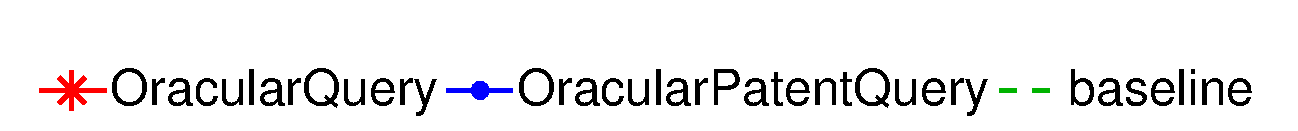
\includegraphics[width=9cm]{imgs/l1}
\par\end{centering}

\begin{centering}
\subfigure[{}\label{fig:lang-a}]{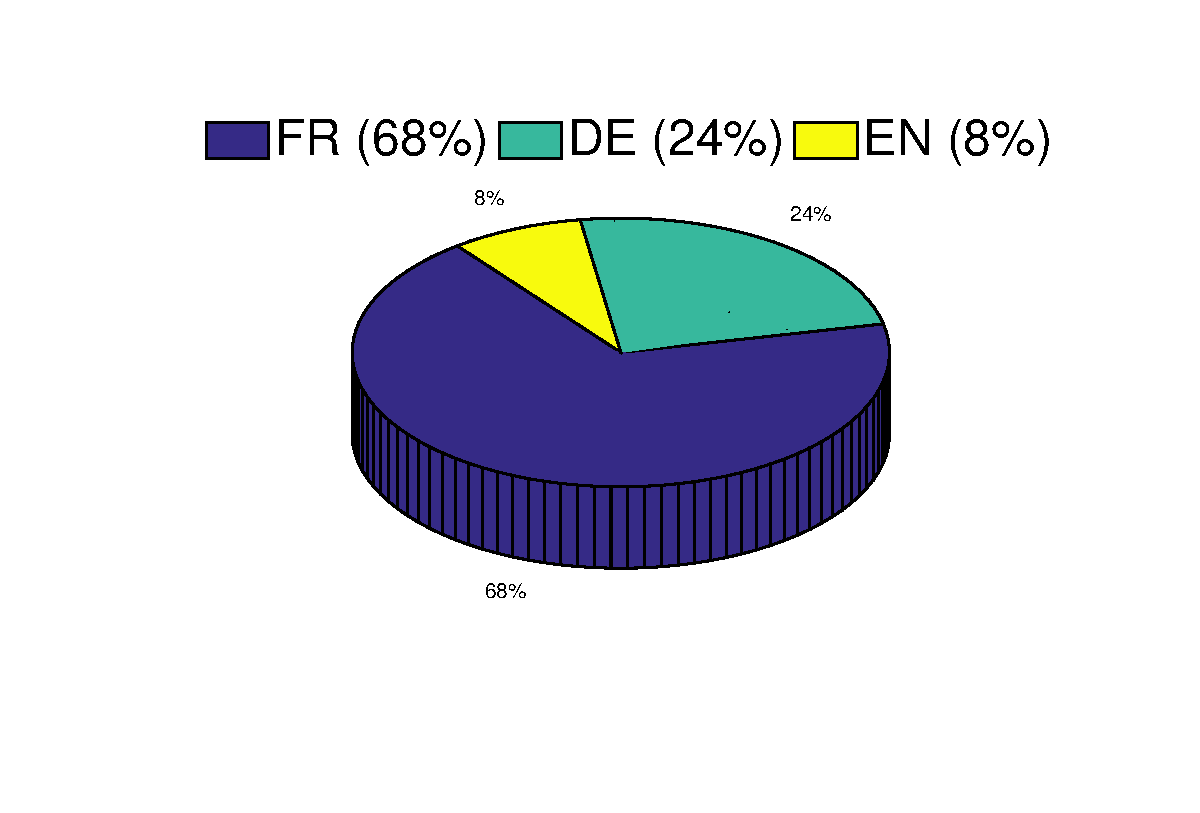
\includegraphics[width=8cm]{figs/lang1.eps}}\subfigure[\label{fig:lang-b}]{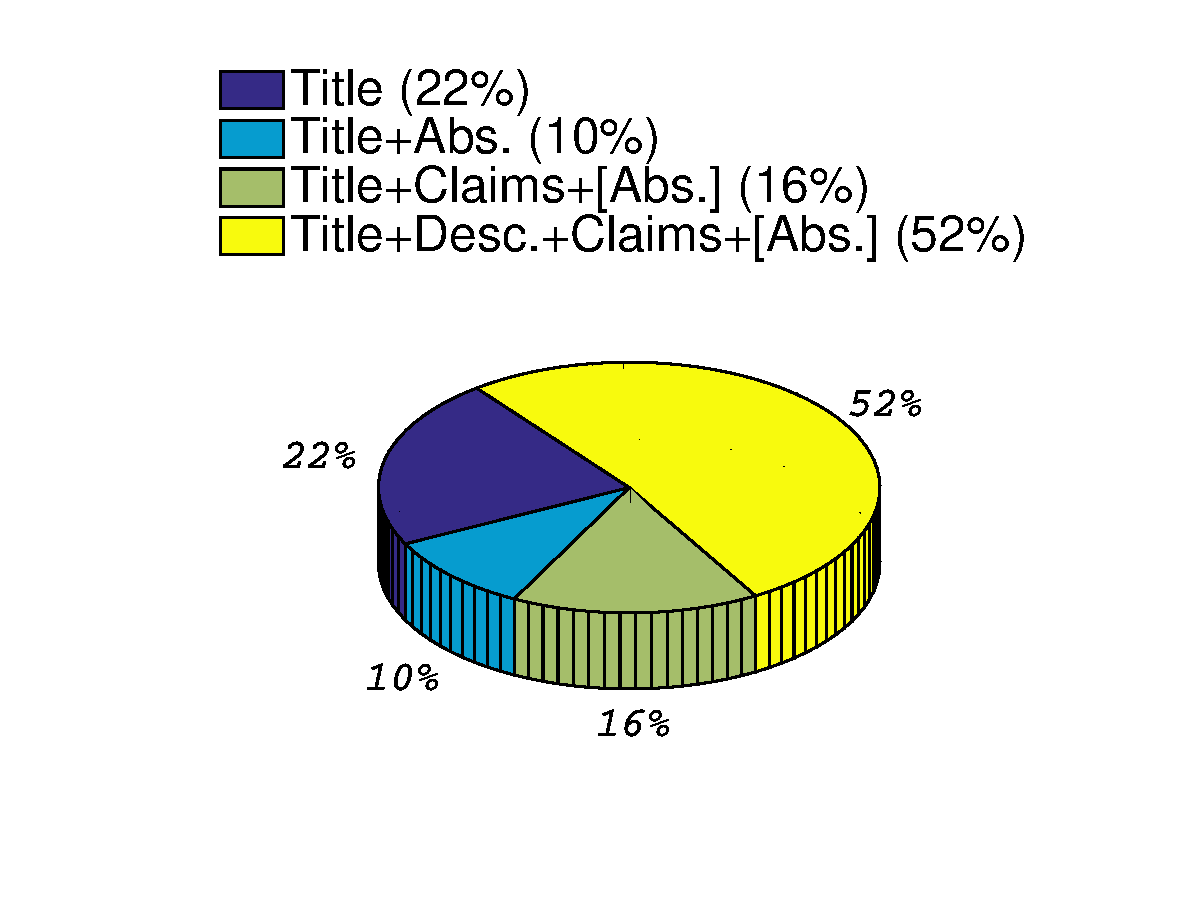
\includegraphics[width=8cm]{figs/lang2.eps}}
\par\end{centering}
\vspace{1mm}
\protect\caption{(a) Percentage of English, German, and French patents in CLEF-IP 2010 collection.
                 (b) Completeness of the presence of English text in the CLEF-IP 2010 patent collection.~\citep{magdy2012toward}.}
\label{fig:lang}
\end{figure}
%%%%%%%%%%%%%%%%%%%%%%%%%%%%%%%%%%%%%%%%%%%%%%%%%%%%%%%%%%%%%%
%\begin{figure}[t!]
%\begin{centering}
%\subfigure[\label{fig:lang-a}]{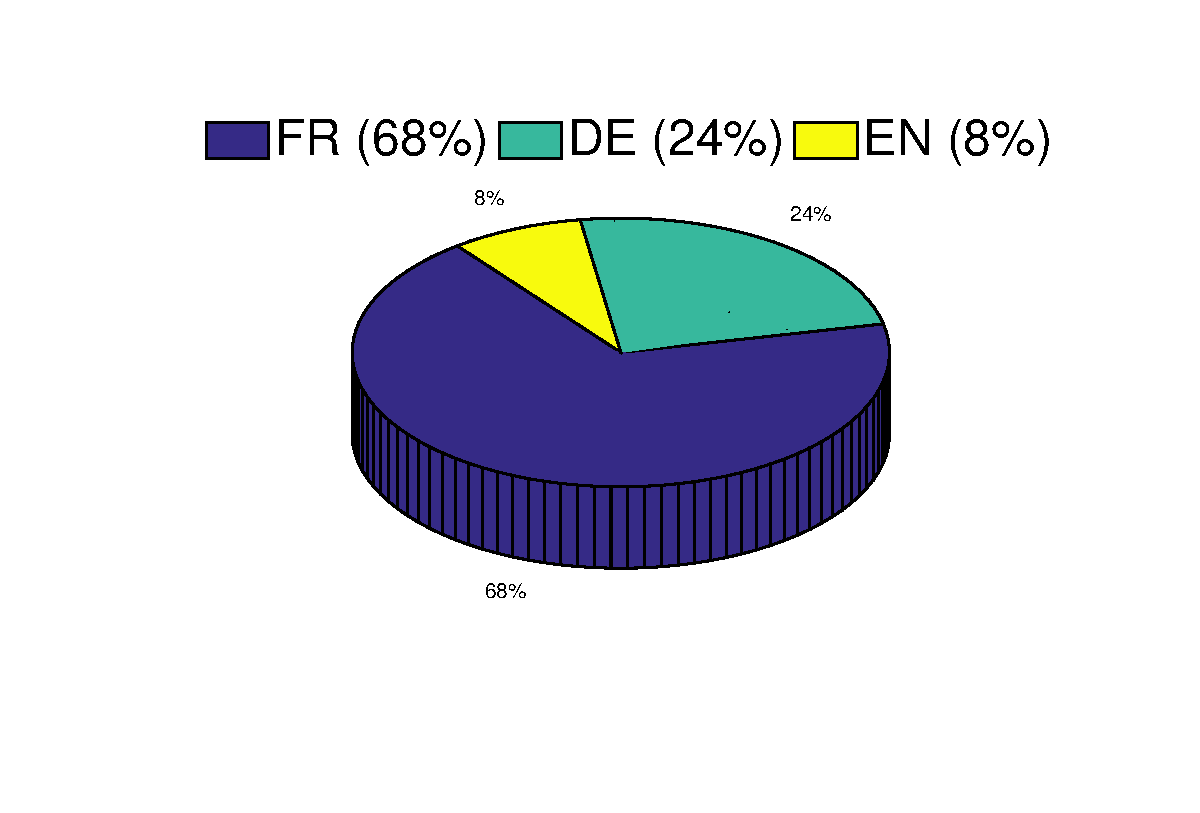
\includegraphics[width=4cm]{figs/lang1.eps}} \hspace*{1.5cm} 
%\subfigure[\label{fig:lang-b}]{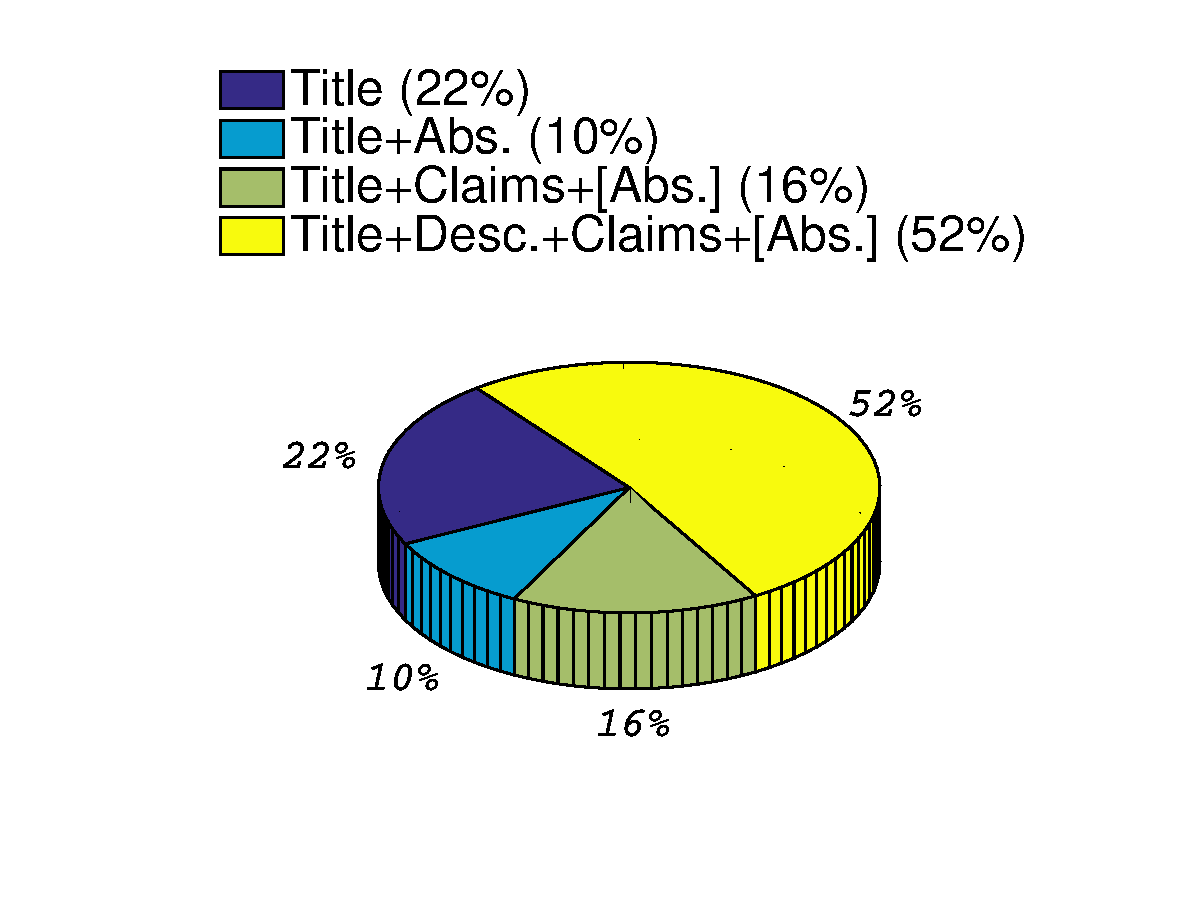
\includegraphics[width=6.5cm]{figs/lang2.eps}} 
%\par\end{centering} 
%\protect\caption{(a) Percentage of English, German, and French patents in CLEF-IP 2010 collection.
%                (b) Completeness of the presence of English text in the CLEF-IP 2010 patent collection.~\citep{magdy2012toward}}
%\label{fig:lang}
%\end{figure}

%%%%%%%%%%%%%%%%%%%%%%%%%%%%%%%%%%%%%%%%%%%%%%%%%%%%%%%%%%%%%%%%
%%%%%%%%%%%%%%%%%%%%%%%%%% Section 3 %%%%%%%%%%%%%%%%%%%%%%%%%%%
%%%%%%%%%%%%%%%%%%%%%%%%%%%%%%%%%%%%%%%%%%%%%%%%%%%%%%%%%%%%%%%%
\section{Errors Caused by Baseline Settings}
Data curation and IPC filter used in baseline settings are two sources of errors;
in this section, we will discuss these two origins of the errors.

\subsection{Data Curation Errors}
\label{sec:DataCurationErrors}
%\vspace{-2mm} 
%CLEF-IP collection has two main characteristics that leads in two main causes of the error: 
Our baseline system cannot retrieve some relevant patent documents because of two main characteristic of CLEF-IP data collection: 
\begin{enumerate}

\item \textbf{Missing description: } As we described in Section~\ref{sec:DataCollection}, some patents in the union collection lose the contents of some sections due to merging different versions of patents. Therefore, relevant patents with missing description are not retrieved by our system.
\item \textbf{Non-English relevant patents: } CLEF-IP data collection has been designed for a multilingual patent search and it consists of patents in three different languages: English, German, and French. However, our baseline $\mathit{IR}$ system is not designed for multilingual search and it cannot retrieve non-English relevant patents.   
\end{enumerate}
%%%%%%%%%%%%%%%%%%%%%%%%%%%%%%%%%%%%%%%%%%%%%%%%%%%%%%%%%%%%%%
\begin{figure}[t!]
\begin{centering}
\subfigure[Cut-off rank ($k$) $= 100$\label{fig:datacuration_a}]{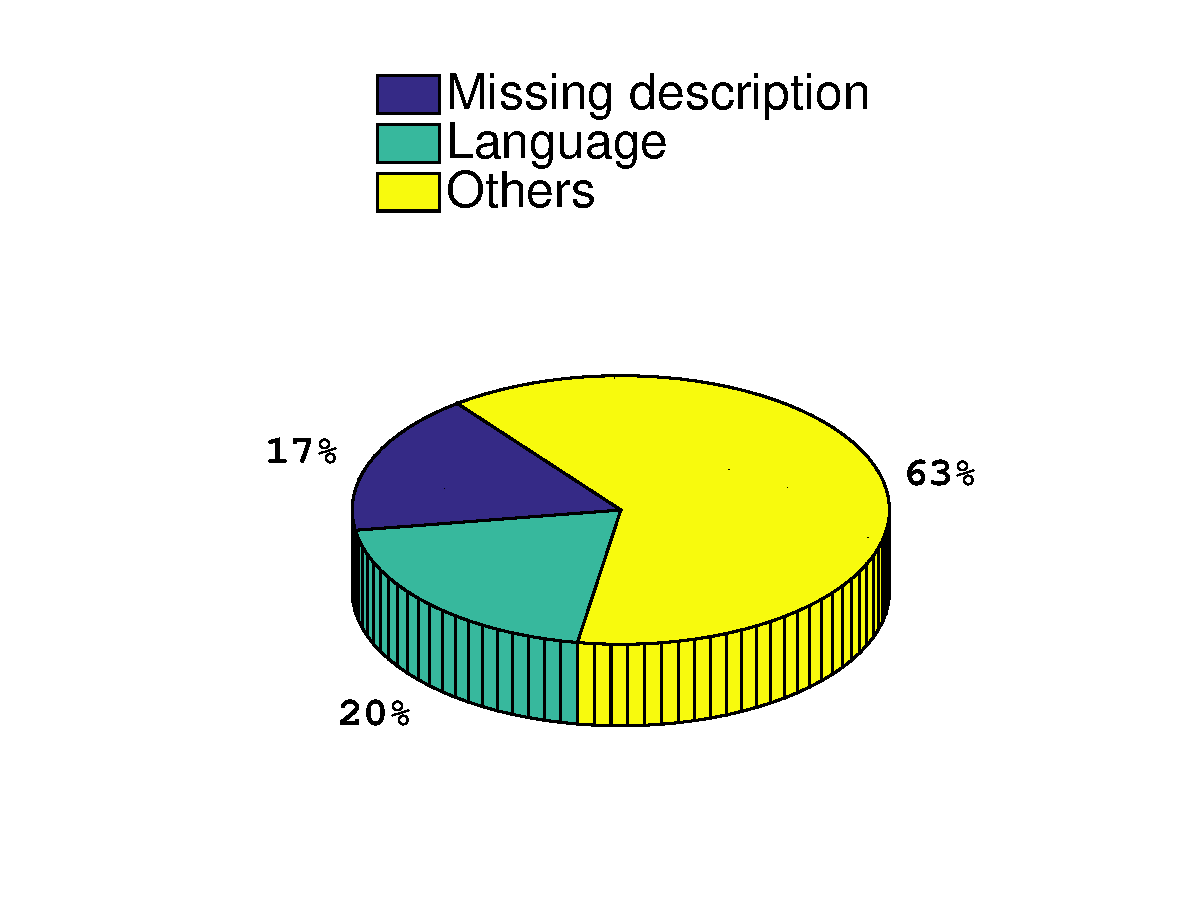
\includegraphics[width=6.5cm]{figs/analyseFNs100.eps}}  
\subfigure[Cut-off rank ($k$) $= 1,000$\label{fig:datacuration_b}]{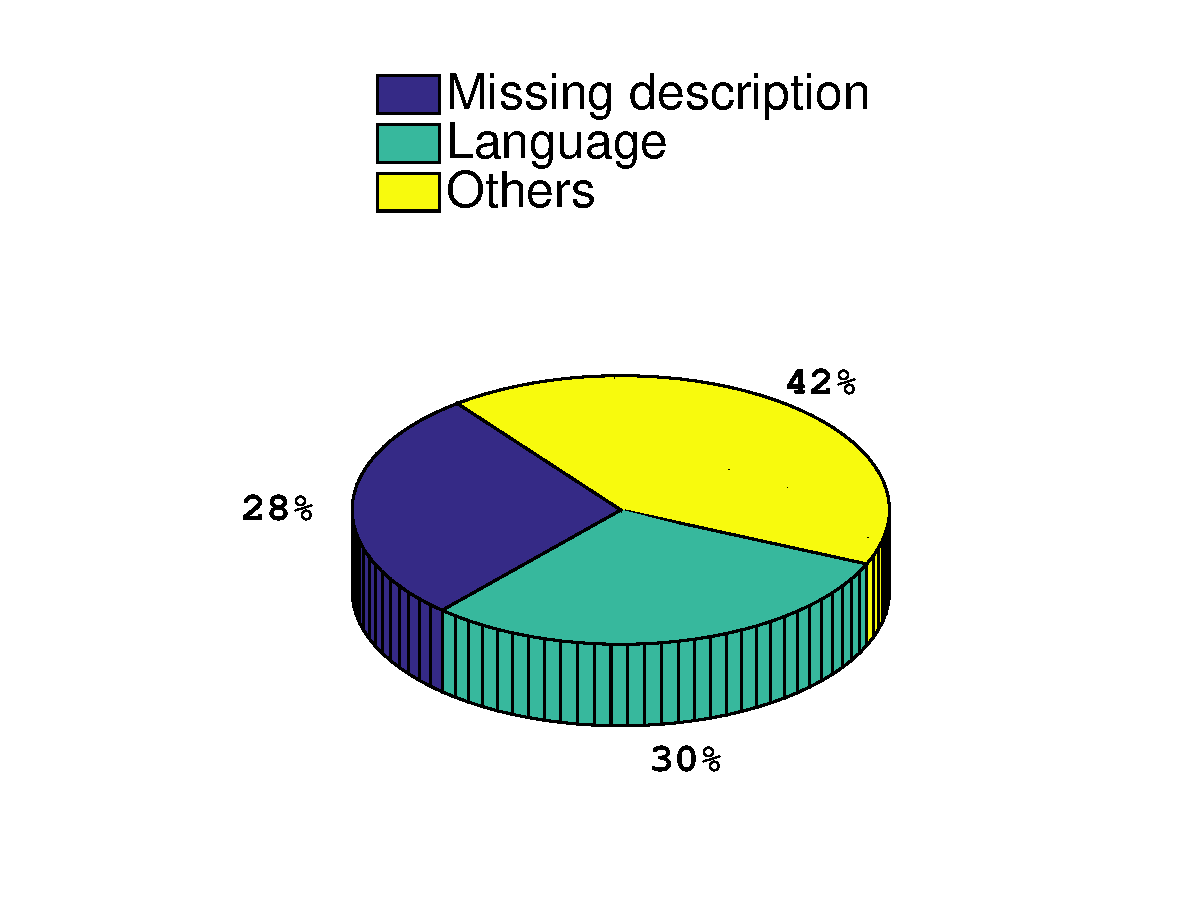
\includegraphics[width=6.5cm]{figs/analyseFNs1000.eps}} 
\par\end{centering} 
\protect\caption{Average percentage of errors due to missing description, language. Overall, $37\%$ of errors are because of data curation while $63\%$ of English complete patent documents cannot be retrieved. Increasing $k$ from $100$ to $1,000$ reduces the errors of the yellow area, but the value of $42\%$ is still notable.}
\label{fig:datacuration}
\end{figure}
%%%%%%%%%%%%%%%%%%%%%%%%%%%%%%%%%%%%%%%%%%%%%%%%%%%%%%%%%%%%%%
We calculate the percentage of errors caused by data curation in this experiment. As it has been illustrated in Figure \ref{fig:datacuration_a}
, overall, $37\%$ of errors are due to CLEF-IP data curation (missing description and non-English relevant patents) while the majority of relevant patents, which are not retrieved ($63\%$), are full English patent documents (Figure \ref{fig:datacuration}). These results indicates that the baseline retrieval system is ineffective to retrieve the majority of the relevant patents because of other reasons. In this research, we are interested in the other reasons that result in low effectiveness of general IR techniques in patent domain. Figure \ref{fig:datacuration_b} shows that by increasing the cut-off rank to $1,000$, still considerable percentage of full English relevant patents --- about $42\%$ --- are not retrieved.








%In this section, we focus on analysing not retrieved relevant (False Negative (FN)) patents. 
%%\vspace{-2mm} 
%CLEF-IP collection has two main characteristics that leads in two main causes of the error: 
%\begin{enumerate}
%\item \textit{Missing `Description': } Each patent in the collection consisted of multiple versions of documents in XML format labelled as $ A_{1} $, $ A_{2} $ ... $ B_{1} $, and $ B_{2} $. The letter `A' refers to different versions of patent applications. The `B' versions refer to granted patents. We merged different versions of a single patent into one union document as recommended by CLEF-IP%
%\footnote{\texttt{\url{http://www.ifs.tuwien.ac.at/~clef-ip/}}%
%}~\citep{magdy2012toward}. As a result of the merging, some patents in the union collection appears with many missing content fields. Since the `Description' is the longest section in a patent, almost, relevant patent with missing `Description' are not retrieved by the baseline.
%\item \textit{Non-English Patents: } The CLEF-IP has been designed for a multilingual patent search and it consists of patents in three different languages: English, German, and French. All patents have the title in the three languages while just the granted published version of a patent(`B' version) by the EPO should contain the claims section manually translated into all three languages. The description section of all patents is always in the original submission language only. Since the design of the baseline did not consider multilinguality, it can not retrieve relevant but non-English patents.   
%\end{enumerate}
%\noindent Fig.(\ref{fig:datacuration}) shows that, overall, \%37 of errors are due to CLEF-IP collection while \%63 of the errors occurs for full English patent documents.
%%\vspace*{-1ex}
%%\vspace{-3.5mm} 
%%%%%%%%%%%%%%%%%%%%%%%%%%%%%%%%%%%%%%%%%%%%%%%%%%%%%%%%%%%%%%%
%\begin{figure}[t!]
%\begin{centering}
%\subfigure[Cut-off rank(k) = 100\label{fig:datacuration_a}]{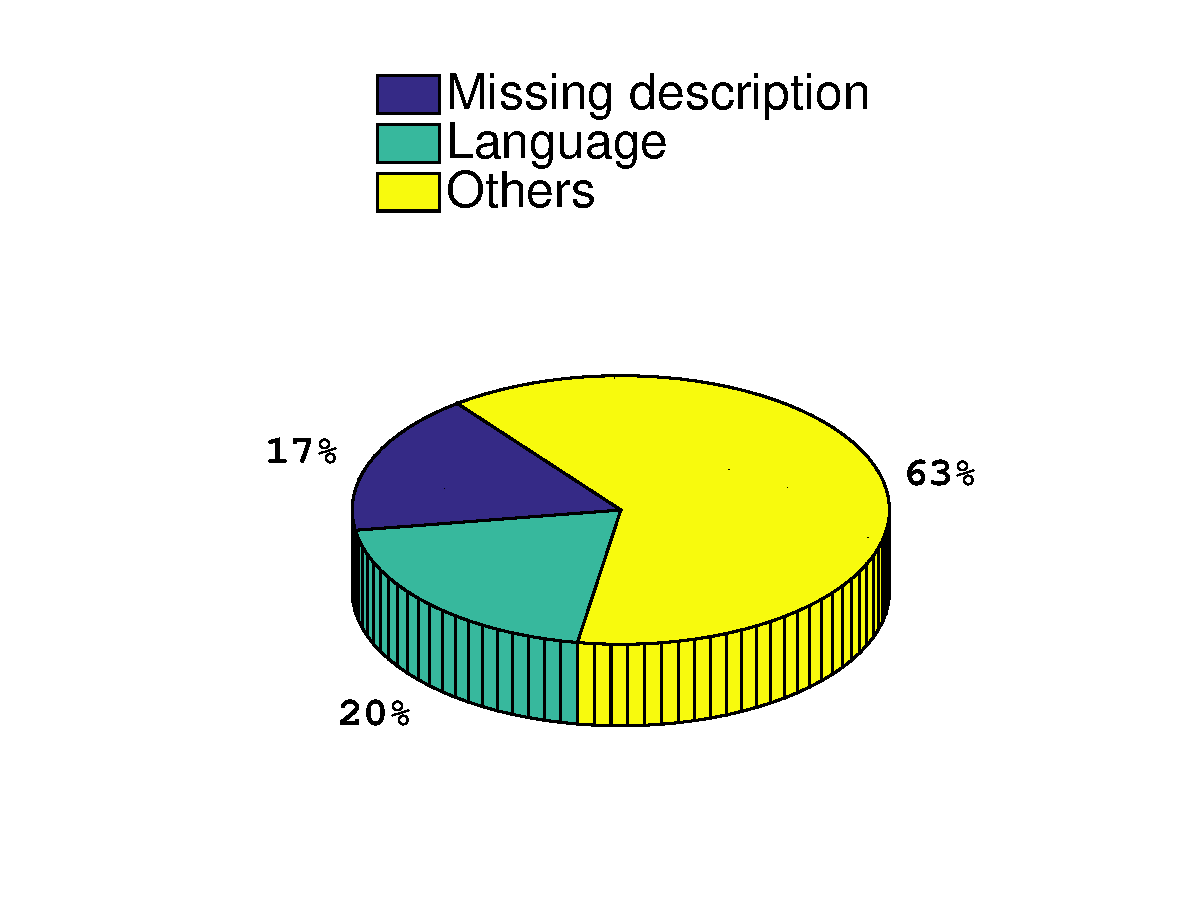
\includegraphics[width=6.5cm]{figs/analyseFNs100.eps}} \hspace*{0.5cm} 
%\subfigure[Cut-off rank(k) = 1000\label{fig:datacuration_b}]{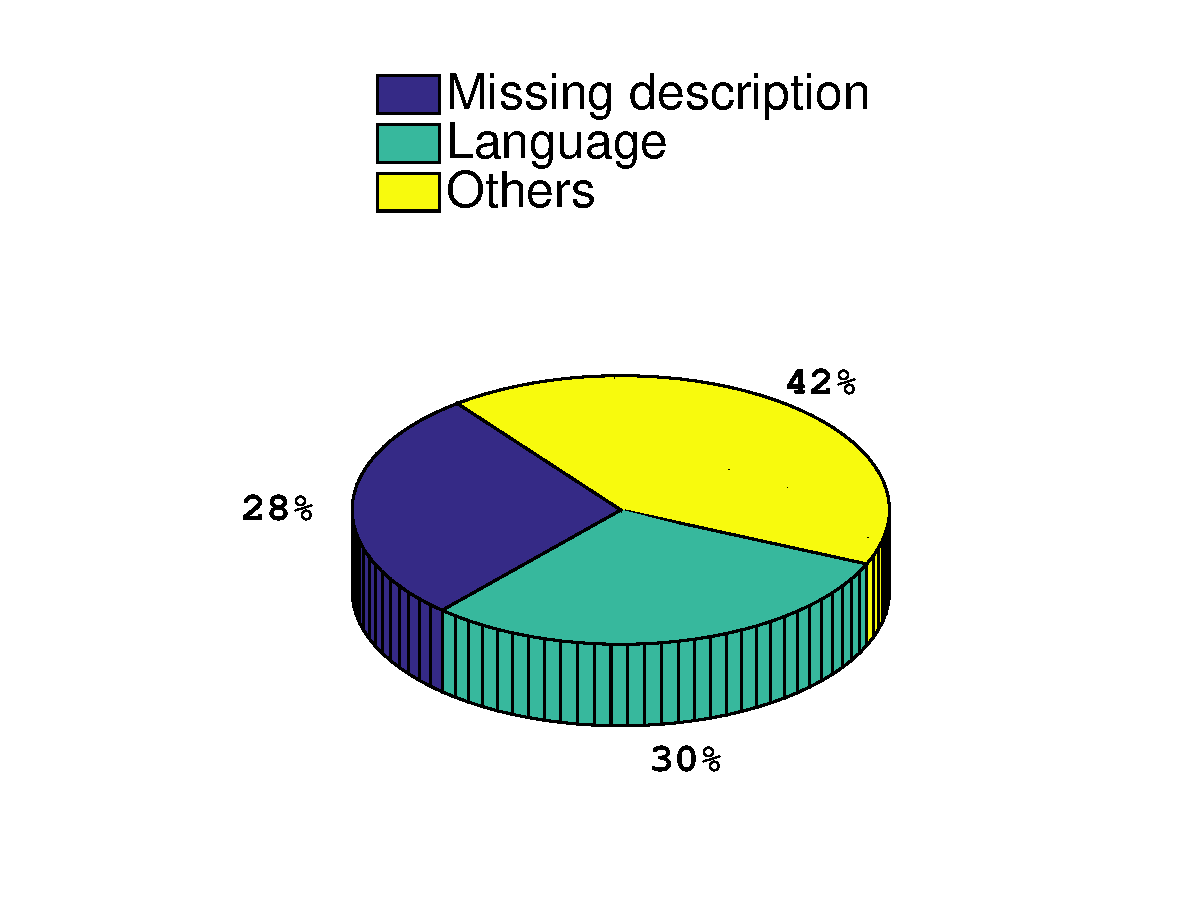
\includegraphics[width=6.5cm]{figs/analyseFNs1000.eps}} 
%\par\end{centering} 
%\protect\caption{Average percentage of errors due to missing `Description', non-English original language. Overall, 37\% of errors are because of data curation while \%63 of English complete patent documents can not be retrieved. Increasing k from 100 to 1000 reduces the errors of red area, but 42\% is still notable.}
%\label{fig:datacuration}
%\end{figure}
%%%%%%%%%%%%%%%%%%%%%%%%%%%%%%%%%%%%%%%%%%%%%%%%%%%%%%%%%%%%%%%
%%\begin{figure}[htpb]
%%%\vspace{2.5cm}
%%\centering
%%\begin{subfigure}[htpb]{.5\linewidth}
%%\centering
%%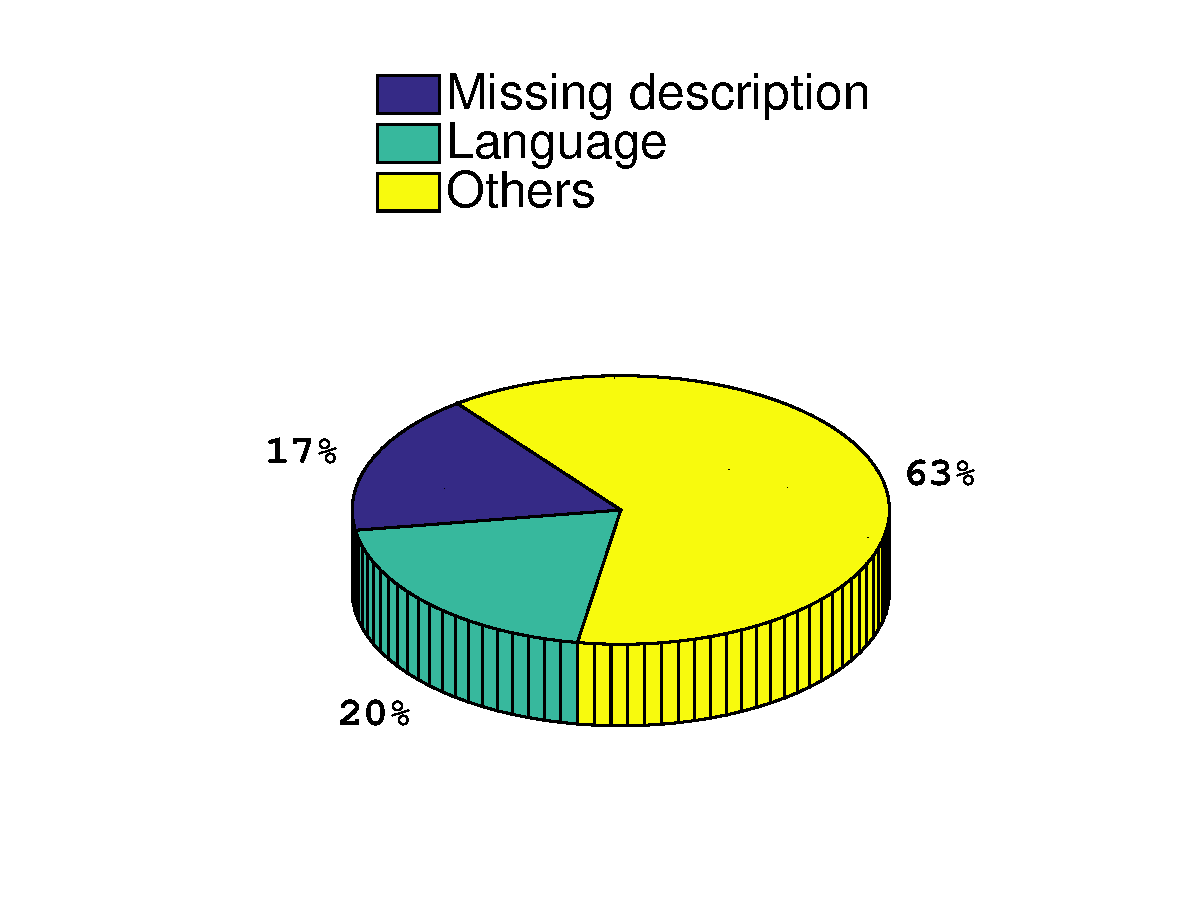
\includegraphics[width=1\textwidth,height=45mm]{figs/analyseFNs100.eps}
%%\caption{Cut-off rank(k) = 100}
%%\label{fig:datacurationk100}
%%\end{subfigure}%\\[1ex]%
%%\begin{subfigure}[htpb]{.5\linewidth}
%%\centering
%%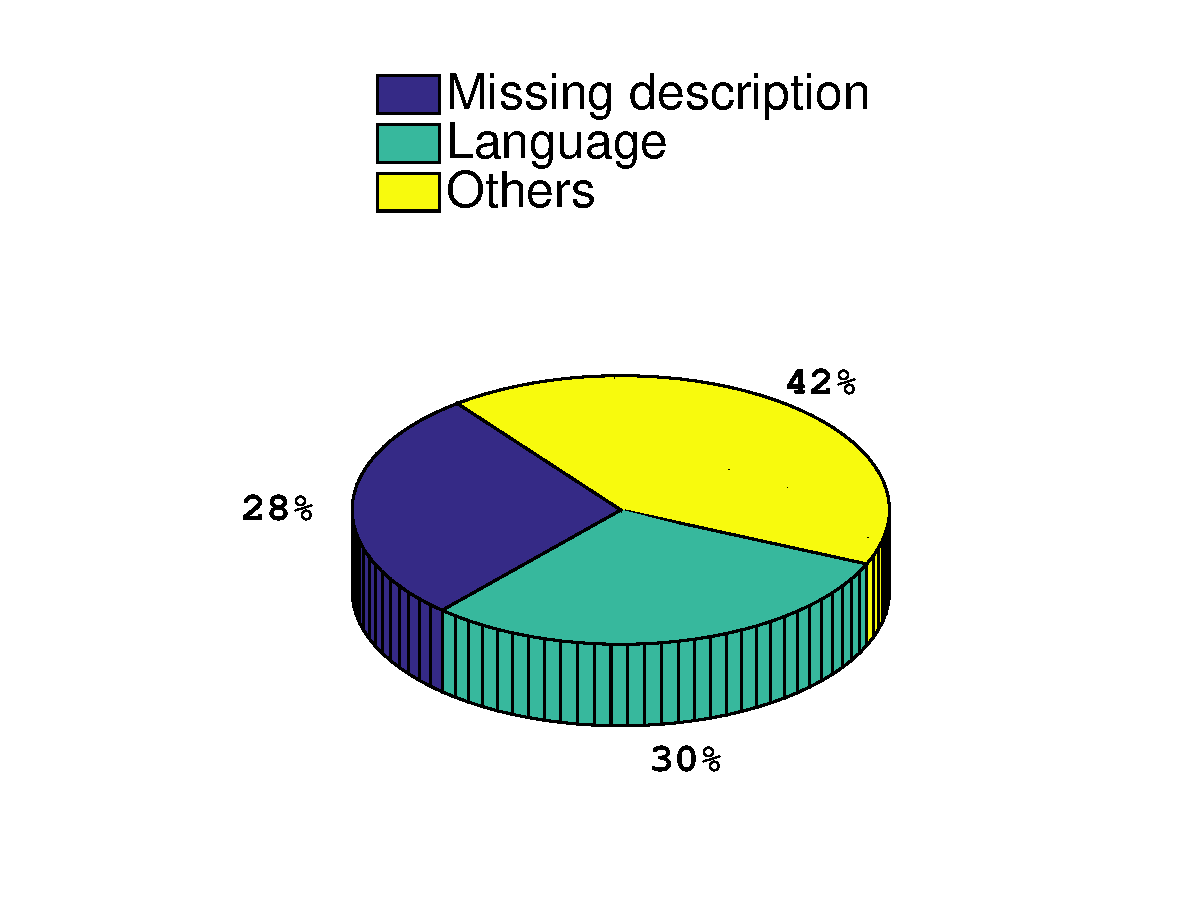
\includegraphics[width=1\textwidth,height=45mm]{figs/analyseFNs1000.eps}
%%\caption{Cut-off rank(k) = 1000}
%%\label{fig:datacurationk100}
%%\end{subfigure}
%%\caption{Average percentage of errors due to missing `Description', non-English original language. Overall, \%37 of errors are because of data curation while \%63 of English complete patent documents can not be retrieved. Increasing k from 100 to 1000 reduces the errors of red area, but \%42 is still notable.}
%%\label{fig:datacuration}
%%\end{figure}
%%\FloatBarrier
%%\noindent
%
%%Table \ref{tab:FNs} compares the average percentage of relevant patents which are not retrieved at top 100, 200, and 1000. 
%%\begin{table*}[htpb]
%%  \begin{center}
%%  \input table/FNs.tex  
%%  \caption{The percentage of relevant documents which are not retrieved at top 100, k= 100, over all test queries. In average, \%57 of relevant patents can not be retrieved by the system at top 100.}
%%  \label{tab:FNs}
%%  \end{center}  
%%\end{table*}
%%\FloatBarrier 
%%\noindent
%
%
%%We categorised the source of failure in three groups:
%%\begin{enumerate}
%%\item patents with missing description.
%%\item patents with non-English original language.
%%\item others: patents which are complete and their original language is English. The reason that they are not retrieved is still unknown, but our hypothesis is that these patents can not be retrieved because they have less term overlap with their related query. 
%%%containing the least term overlap with the query.
%%\end{enumerate}
%%The two first groups are the characteristic of our collection and we are not interested in improve the baseline to retrieve them. Whereas, we are interested in improve our system to be able to retrieve the third group.
%%Figure \ref{fig:failingCategory} shows the percentage of each failure source averaged over all queries in FN subset (k = 100).
%%\begin{figure}[htpb]
%%   \centering
%%   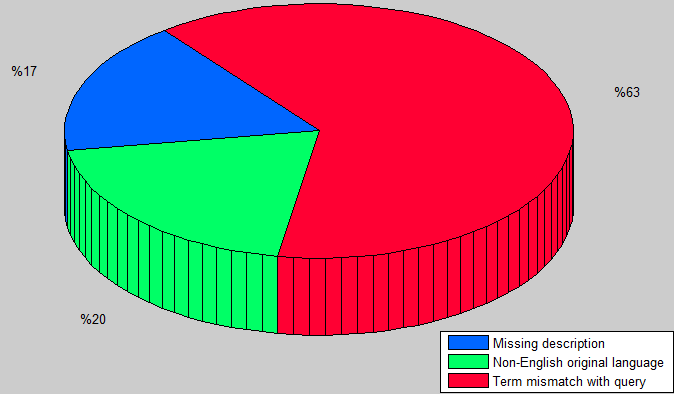
\includegraphics[width=0.55\textwidth,height=45mm]{figs/failingCategory.png}
%%   \caption{Average percentage of patents with missing description, non-English original language, and term mismatch with the query in FN patents over all queries.(k=100).}  
%%   \label{fig:failingCategory} 
%%\end{figure}
%%\FloatBarrier 
%%\noindent
%
%By increasing the ranking threshold to 1000, the percentage of term mismatch failure source decreases in FN subset; Whereas, \%41 is still considerable. 
%
%%\begin{figure}[htpb]
%%   \centering
%%   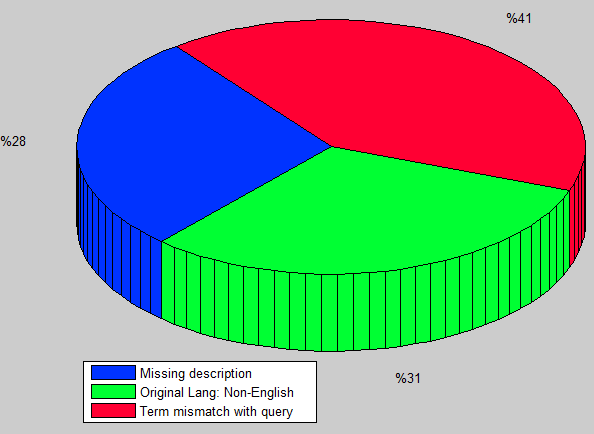
\includegraphics[width=0.55\textwidth,height=55mm]{figs/FNs-k1000.png}
%%   \caption{Average percentage of patents with missing description, non-English original language, and term mismatch with the query in FN patents over all queries.(k=1000).}  
%%   \label{fig:FNs-k1000} 
%%\end{figure}
%%\FloatBarrier 
%%\noindent
%
%We can conclude from Fig. \ref{fig:datacuration} that the main reason, which relevant documents are not retrieved, is the term mismatch between the query and relevant patents,  even in top 1000 documents. The portion of missing description and non-English original language are also high enough to deteriorate the system performance. In our research, we focus on term mismatch between query and relevant documents not missing description or multilinguality which are specific to clef-ip data collection.
%
%Our detailed results also indicate that by increasing the ranking threshold from 100 to 1000, the number of false negatives due to term mismatch between query and relevant documents decreased. Whereas there are some queries that their relevant patents in English do not retrieve even at the rank 1000. 
%
%The focus of this research is to identify the reasons that the system fails to retrieve patents in the red area, where the patents are complete English documents. Hence, in the rest of this paper, we continue our experiment in the red area.\\\\
%\textbf{Anecdotal Examples}\\
%In following experiments, we selected five sample queries from the category: "other"; The following figures show the query term frequency in relevant not-retrieved patents. 
%\begin{landscape}
%\begin{figure}[htpb]
%   \centering
%   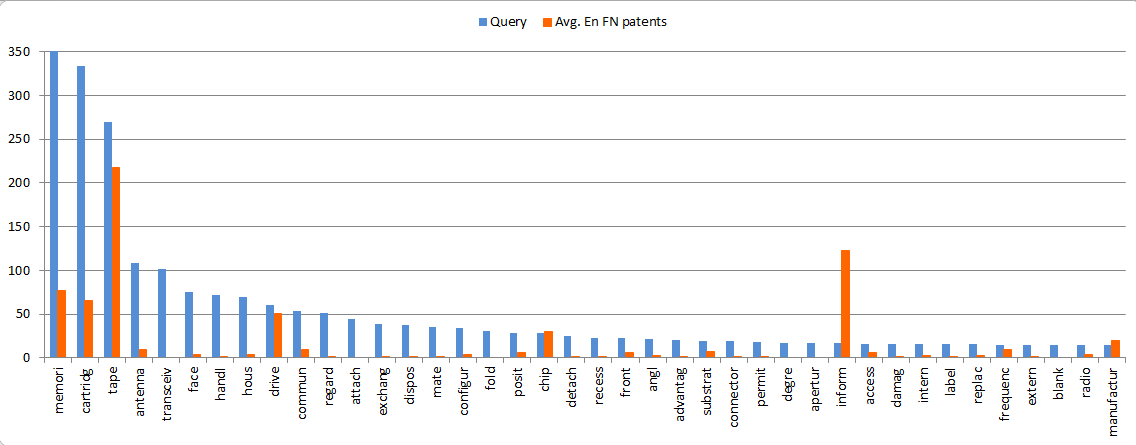
\includegraphics[width=\columnwidth,height=100mm]{figs/pac1035-avgEnFNs.png}
%   \caption{Comparing term frequencies in query, and average term frequencies in relevant not-retrieved patents for Query: PAC-1035. 6/8 patents which are also English can not be retrieved before rank 100, but all can be retrieved before the rank 1000. This indicates that although there is few overlap between query and relevant patents, they will be retrieved but at higher ranks after 100.} 
%   \label{fig:fn-pac1035} 
%\end{figure}
%\end{landscape}
%\FloatBarrier
%\noindent
%  
%\begin{landscape}
%\begin{figure}[htpb]
%   \centering
%   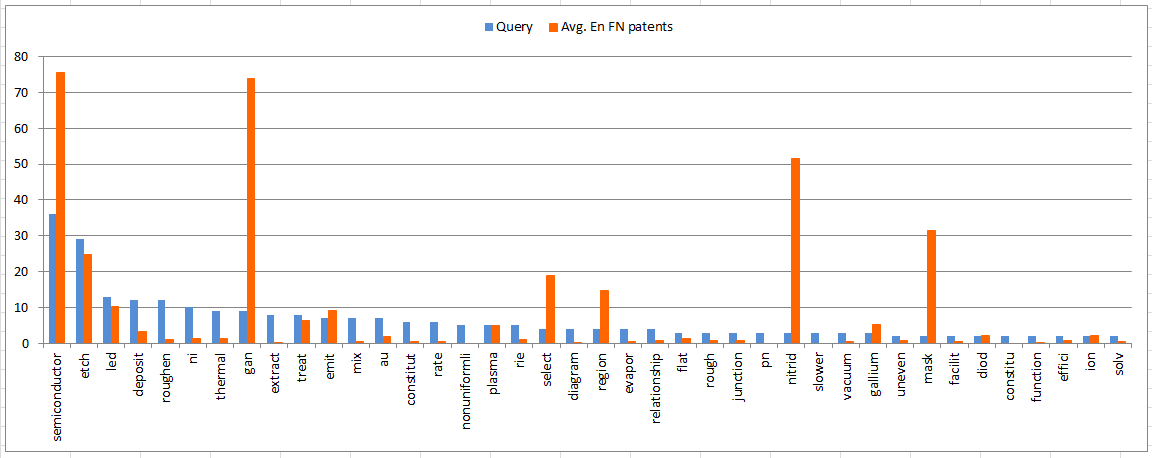
\includegraphics[width=\columnwidth,height=100mm]{figs/fn-pac1142.png}
%   \caption{Comparing term frequencies in query, and average term frequencies in relevant not-retrieved patents for Query: PAC-1142. (En FNs)/FNs = 9/10, @ k=100, and still (En FNs)/FNs = 7/10 @ k=1000. This indicates that 7 relevant patents for this query are not retrievable.} 
%   \label{fig:fn-pac1142} 
%\end{figure}
%\end{landscape}
%\FloatBarrier
%\noindent
%
%\begin{landscape}
%\begin{figure}[htpb]
%   \centering
%   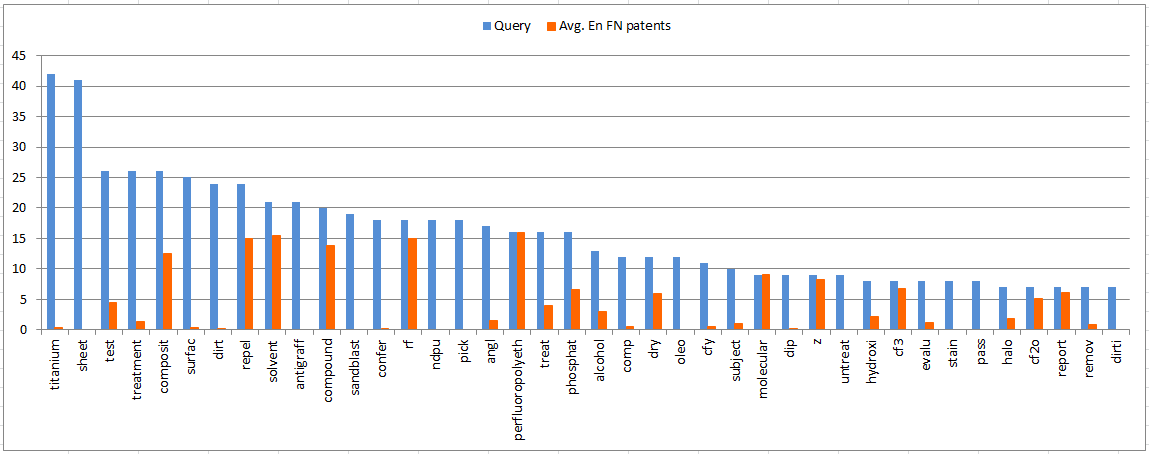
\includegraphics[width=\columnwidth,height=100mm]{figs/fn-pac1216.png}
%   \caption{Comparing term frequencies in query, and average term frequencies in relevant not-retrieved patents for Query: PAC-1216. This query is an example that its English relevant patents (5/6) can not be retrieved even at rank 1000.} 
%   \label{fig:fn-pac1216} 
%\end{figure}
%\end{landscape}
%\FloatBarrier
%\noindent
%
%\begin{landscape}
%\begin{figure}[htpb]
%   \centering
%   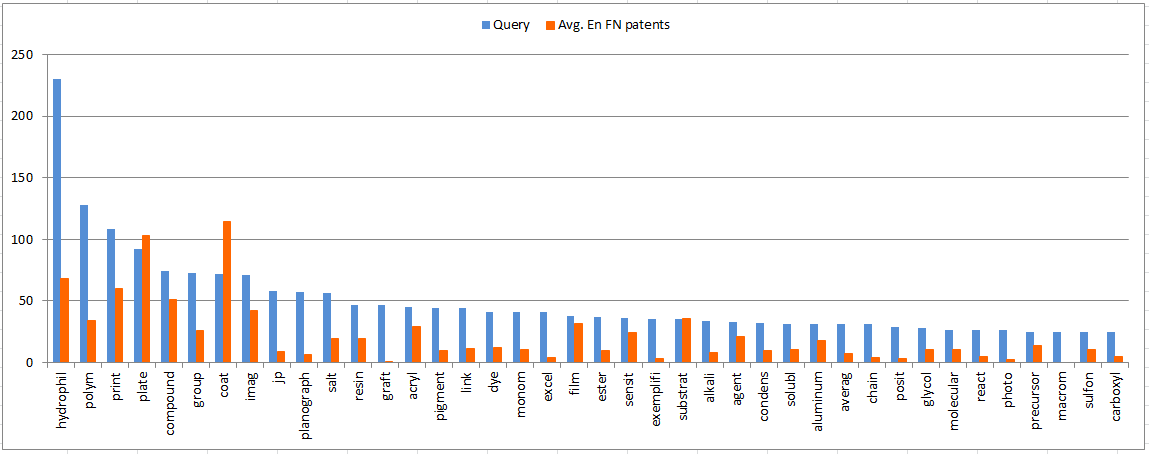
\includegraphics[width=\columnwidth,height=100mm]{figs/fn-pac1379.png}
%   \caption{Comparing term frequencies in query, and average term frequencies in relevant not-retrieved patents for Query: PAC-1379. (En FNs)/FNs = 14/17, @ k=100, and still (En FNs)/FNs = 12/17, @ k=1000. This indicates that 12 English relevant patents for this query are not retrievable.} 
%   \label{fig:fn-pac1379} 
%\end{figure}
%\end{landscape}
%\FloatBarrier
%\noindent
%
%\begin{landscape}
%\begin{figure}[htpb]
%   \centering
%   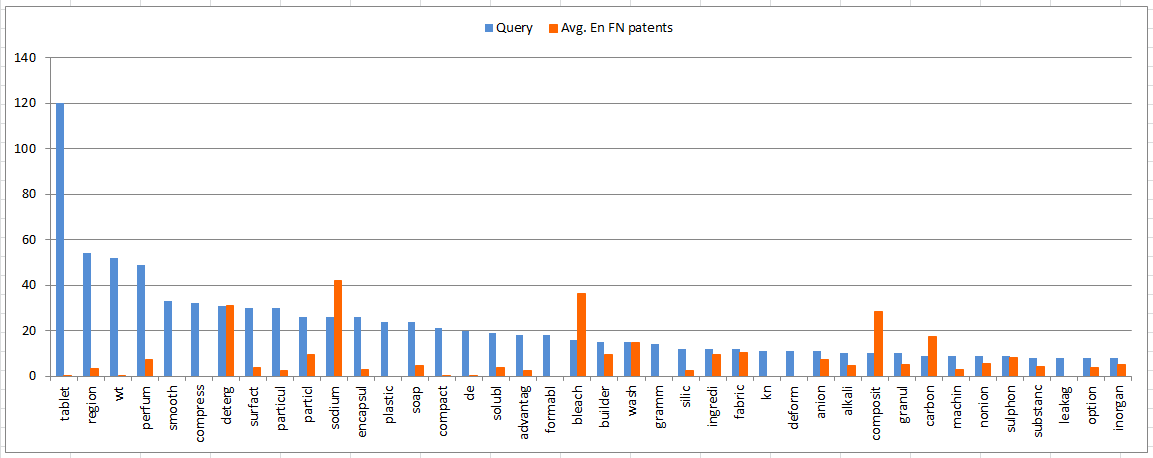
\includegraphics[width=\columnwidth,height=100mm]{figs/fn-pac1604.png}
%   \caption{Comparing term frequencies in query, and average term frequencies in relevant not-retrieved patents for Query: PAC-1604. (En FNs)/FNs = 10/19, @ k=100, and still (En FNs)/FNs = 9/19 @ k=1000. This indicates that 9 English relevant patents for this query are not retrievable.} 
%   \label{fig:fn-pac1604} 
%\end{figure}
%\end{landscape}
%\FloatBarrier
%\noindent
%Our experiments showed the reason that some relevant patents are not retrieved by the system is not that there is zero term overlap between the query and documents, it is low weighting of query terms in the relevant documents. 



%\begin{table*}[htpb]
%  \begin{center}
%  \input table/errorCategory.tex  
%  \caption{Percentage of missing, non-English, and term mismatch error category in FN patents. }
%  \label{tab:threshold}
%  \end{center}  
%\end{table*}
%\FloatBarrier 
%\noindent

%Patent retrieval is a recall-oriented task and it is important to retrieve all relevant patents appear at top of the list. Patent examiners, our users, usually prefer to look at 100-200 top retrieved patents. Table \ref{tab:threshold} shows about \%16 decrease in recall which are not desired for our users. 
%\begin{table*}[htpb]
%  \begin{center}
%  \input table/threshold.tex  
%  \caption{Comparing performance of the baseline by changing the retrieval threshold.}
%  \label{tab:threshold}
%  \end{center}  
%\end{table*}
%\FloatBarrier 
%\noindent
%
%\begin{figure}[htpb]
%   \centering
%   \includegraphics[width=0.65\textwidth,height=65mm]{figs/a1000.png}
%   \caption{Baseline performance variation over all queries (k=1000).}  
%   \label{fig:a1000} 
%\end{figure}
%\FloatBarrier 
%\noindent
%%
%%\begin{figure}[htpb]
%%   \centering
%%   \includegraphics[width=0.65\textwidth,height=65mm]{figs/a100.png}
%%   \caption{Baseline performance variation over all queries (k=100).}  
%%   \label{fig:a100} 
%%\end{figure}
%%\FloatBarrier 
%%\noindent
%
%\begin{figure}[htpb]
%\label{fig:base}
%        \centering
%        \begin{subfigure}[b]{0.6\textwidth}
%        \centering
%                \includegraphics[width=1\textwidth,height=65mm]{figs/a100.png}
%                \caption{ }
%                \label{fig:baseperformancea}
%        \end{subfigure}%
%        ~ %add desired spacing between images, e. g. ~, \quad, \qquad, \hfill etc.
%          %(or a blank line to force the subfigure onto a new line)
%        \begin{subfigure}[b]{0.6\textwidth}
%        \centering
%                \includegraphics[width=1\textwidth,height=65mm]{figs/a1000.png}
%                \caption{ }
%                \label{fig:baseperformanceb}
%        \end{subfigure}
%       \caption{
%                Baseline performance variation over all queries (a) k=1000.
%                (b) k=100.
%                } 
%\end{figure}
%\FloatBarrier
%\noindent
%Figure \ref{fig:baseperformancea} and \ref{fig:baseperformanceb} show the variation of the baseline system performance. Figure \ref{fig:baseperformancea} is when choosing the top rank k = 100 and figure \ref{fig:baseperformanceb} is for k = 1000. It can be seen that 'Recall' and 'PRES' skew up when we increase the rank threshold, but there is no significant improvement for 'Average Precision (AP)' because it is more sensitive to finding relevant documents at very high ranks regardless of the number of documents to be checked by the user. However, 'PRES' is more sensitive to the average ranking of the relevant retrieved documents as a whole relative to the maximum number of documents the user is willing to check. Foe example, when Nmax=1000, the ranks {32, 35, 46} are considered relatively good compared to this number. Nevertheless, when calculating PRES with Nmax=100, the PRES value will be less which represents the average ranking of the relevant documents relative to the maximum number of documents to be checked. Low 'AP' indicates that system is also incapable of retrieving patents at top of the list with high ranks. The reason was indicated in previous section (term level analysis), irrelevant patents have more common words with the query which ends in retrieving them at top of the list. The solution is finding the noisy words which appear more in the irrelevant documents and should be identified and removed. 
%%\begin{list}{-}{}
%%\end{list}


%%%%%%%%%%%%%%%%%%%%%%%%%%%%%%%%%%%%%%%%%%%%%%%%%%%%%%%%%%%%%%%%
\subsection{Classification Code Mismatch}
\label{sec:ClassificationCodeMismatch}

%\subsubsection{International Patent Classification code}
%In 1971, the Strasbourg Agreement established the International Patent Classification (IPC) under the World Intellectual Property Organization (WIPO), which divides technology into eight discrete Sections. The goal of this
%Agreement was to overcome the difficulties caused by using diverse national patent classification systems.~\citep{harris2010comparison}
%
%A patent is assigned to one or more of the 71,000 IPC codes that 
%indicate the related technical field or fields the patent covers. 
%These codes are arranged in a hierarchical, tree-like structure with 
%five distinct components. Fig. \ref{fig:ipcexample} illustrates the components of an IPC classification.
%
%The highest hierarchical level contains the eight sections of the IPC corresponding
%to very broad technical fields, labeled A through H. For example, Section C deals
%with``Chemistry and Metallurgy''. Sections are subdivided into classes. The eighth edition of the IPC contains 120
%classes. Class C07, for example, deals with ``Organic Chemistry''. Classes are further subdivided into more than 600 subclasses. Subclass C07C, for example, deals with ``Acyclic or Carbocyclic Compounds''. Subclasses are then further divided into main groups and subgroups. Main group symbols end with ``/00''. Ten percent of all IPC groups are main
%groups. For example, main group C07C 35/00 deals with ``Compounds having at
%least one hydroxy or O-metal group bound to a carbon atom of a ring other than
%a six-membered aromatic ring''. In some versions of the IPC, a series of numbers will follow the subgroup, reflecting
%the enactment date of the IPC version. `20060101' following the Subgroup
%indicates a date of January 1, 2006, which is the date that the eighth version of
%the IPC took effect. 
%%%%%%%%%%%%%%%%%%%%%%%%%%%%%%%%%%%%%%%%%%%%%%%%%%%%%%%%%%%%%%%%%%%%%%%%%%%%%%%%%%
%\begin{figure}[t!]
%   \centering
%   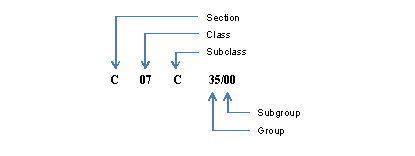
\includegraphics[width=0.70\textwidth,height=35mm]{figs/IPCexample.jpg}
%   \caption{An example illustrating the components of an International Patent Classification code.}   
%   \label{fig:ipcexample} 
%\end{figure}
%%%%%%%%%%%%%%%%%%%%%%%%%%%%%%%%%%%%%%%%%%%%%%%%%%%%%%%%%%%%%%%%%%%%%%%%%%%%%%%%%%
%\subsubsection{IPC Classification as a Filter}
As we mentioned in Section~\ref{sec:settings}, IPC codes (Section~\ref{StructureofPatents}) 
are assigned to patent queries to filter the search results by constraining them to have common IPC codes with the patent query.
In this section, we investigate the errors caused by classification code mismatch between topics (queries) and relevant documents for three different level of hierarchy. 
 
%\subsubsection{Applying 4-digit IPC code for filtering}
%\label{subsec: 4-digit}
\paragraph{Filter Type I: Three First Components of IPC Code}
\ \\
First, we examine the effect of filtering out the patents, which their three first symbols of IPC code, including section, class, and subclass (e.g., $\mathit{C07C}$ in Figure~\ref{fig:ipcexample}), do not match with the patent query. We have applied this filter to our baseline system. As a consequence, relevant patents, which do not share these three symbols of the IPC code with the patent query, are not retrieved by the system.   

Our experiments show that   
around 19\% of the not-retrieved relevant patents do not share any IPC code with the patent query, but the majority of them have main IPC code of the query, and about 21\% have, at least, one of the further IPC codes of the query (Figure~\ref{fig:ipcoverlap_a}). 
%%%%%%%%%%%%%%%%%%%%%%%%%%%%%%%%%%%%%%%%%%%%%%%%%%%%%%%%%%%%%%%%%%%%%%%%%%%%%%%%%
%\begin{figure}[t!]
%   \centering
%   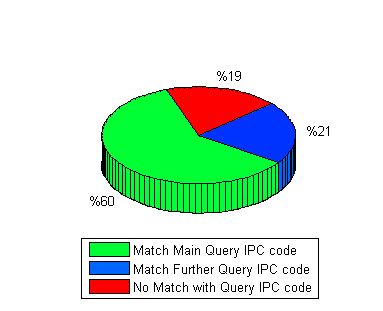
\includegraphics[width=0.60\textwidth,height=69mm]{figs/ipcOverlap-FNs.png}
%   \caption{Classification code overlap between the query and non-relevant retrieved patents (False Negative (FN) patents).}   
%   \label{fig:fnipcoverlap} 
%\end{figure}
%%%%%%%%%%%%%%%%%%%%%%%%%%%%%%%%%%%%%%%%%%%%%%%%%%%%%%%%%%%%%%%%%%%%%%%%%%%%%%%%%
%%%%%%%%%%%%%%%%%%%%%%%%%%%%%%%%%%%%%%%%%%%%%%%%%%%%%%%%%%%%%%
\begin{figure}[t!]
\begin{centering}
\subfigure[Not-retrieved relevant patents (False Negative (FN) patents)\label{fig:ipcoverlap_a}]{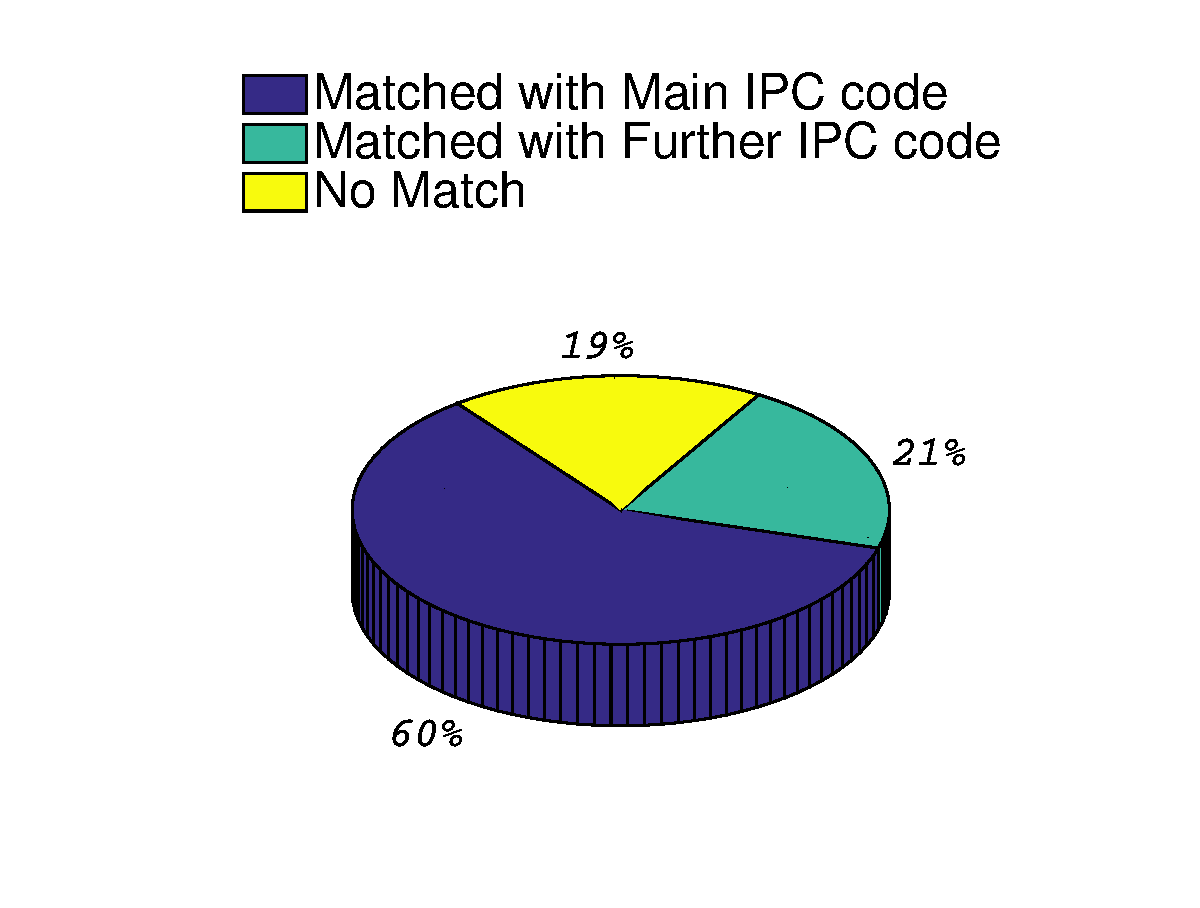
\includegraphics[width=6.5cm]{figs/ipcOverlap-FNs.eps}} 
\hspace*{0.5cm}  \subfigure[Retrieved relevant patents (True Positive (TP) patents)\label{fig:ipcoverlap_b}]{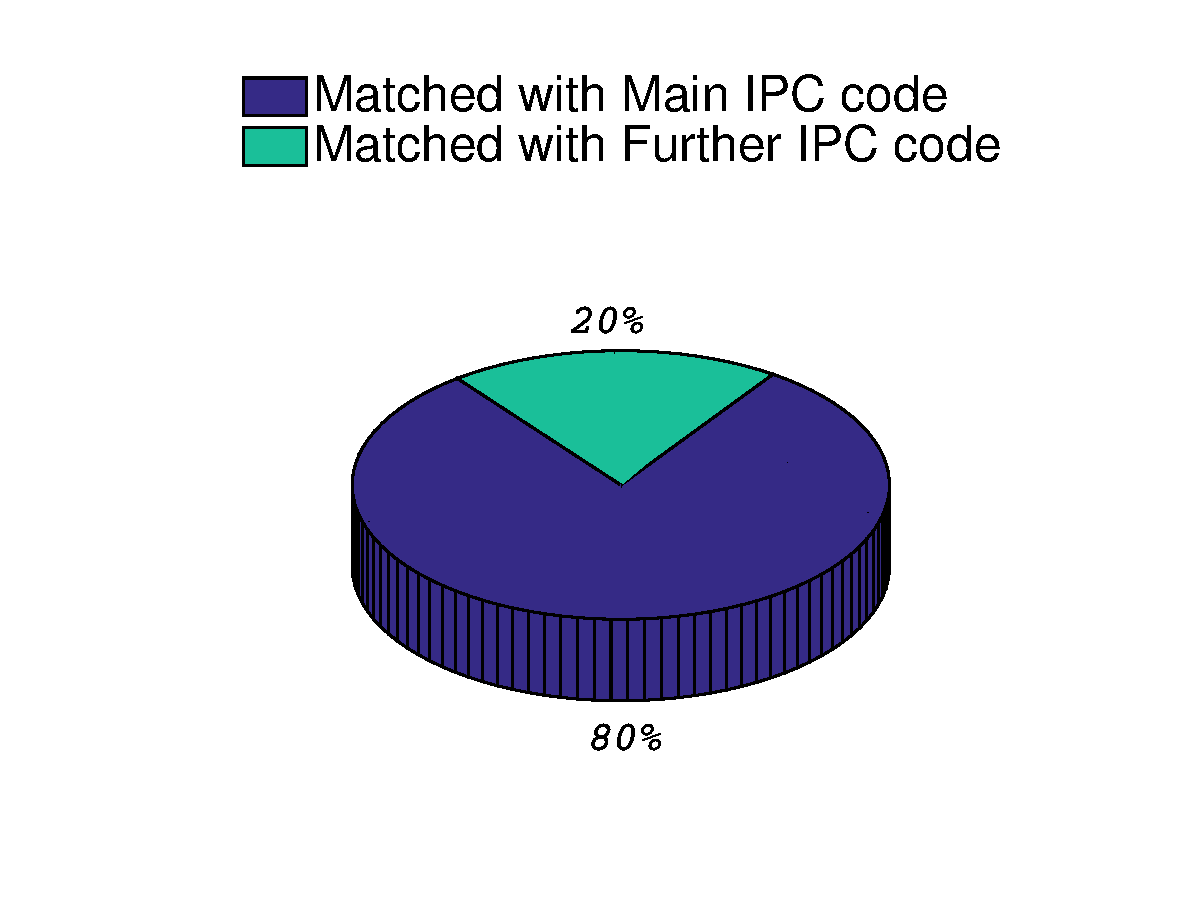
\includegraphics[width=6.5cm]{figs/ipcOverlap-TPs.eps}} 

\par\end{centering} 
\protect\caption{Classification code overlap between the query and non-relevant retrieved patents (False Negative (FN) patents).}
\label{fig:ipcoverlap}
\end{figure}
%%%%%%%%%%%%%%%%%%%%%%%%%%%%%%%%%%%%%%%%%%%%%%%%%%%%%%%%%%%%%%
We repeat the experiments for the true positive (TP) patents; as it has been shown in Figure \ref{fig:ipcoverlap_b}, 80\% of TP patents have an overlap with the main IPC code of the query and 20\% with, at least, one of the query further IPC codes. 
%So, we can conclude that 19\% of errors can be due to IPC filtering if we assume that they have enough term overlap with the query.  
%%%%%%%%%%%%%%%%%%%%%%%%%%%%%%%%%%%%%%%%%%%%%%%%%%%%%%%%%%%%%%%%%%%%%%%%%%%%%%%%%
%\begin{figure}[t!]
%   \centering
%   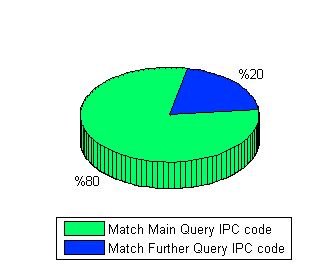
\includegraphics[width=0.55\textwidth,height=60mm]{figs/ipcOverlap-TPs.png}
%   \caption{Classification code overlap between the query and relevant retrieved patents (True Positive (TP) patents).}   
%   \label{fig:tpipcoverlap} 
%\end{figure}
%%%%%%%%%%%%%%%%%%%%%%%%%%%%%%%%%%%%%%%%%%%%%%%%%%%%%%%%%%%%%%%%%%%%%%%%%%%%%%%%%
Although we cannot retrieve around 19\% of relevant patents as a result of applying the IPC filter, we still keep using the filter in our experiments for the following two main reasons: 
\begin{enumerate}
\item CLEF-IP 2010 collection contains 2.6 million patent documents. If we do not use the IPC filter, it will take long time to compare each patent in the whole collection with the query. Nonetheless, if we apply the filter, this process will take faster because the matching process is done on only the portion of the collection, which shares an IPC code with the patent query not the whole collection. Since only less than 19\% of errors are due to a classification mismatch, we continue our analysis by keeping the filter on. The matching process is computationally much faster when we apply the IPC filter. In trade off between losing the percentage of the relevant patents and faster computation, we choose the efficient computation. The computational time is critical in patent prior art search because the query is the description of the the patent query, consisting of thousands of words.   
\item The precision in the top $k$ (100) significantly drops, when we rank the whole collection versus only a subset of patents that have the same classification code with the patent query.  
\end{enumerate}

We conduct the following experiment to justify the first above-mentioned reason. First, we calculate the number of documents that should be processed during the ranking process per query after applying the filter. Then we plot the distribution of this number over all test topics.
%%%%%%%%%%%%%%%%%%%%%%%%%%%%%%%%%%%%%%%%%%%%%%%%%%%%%%%%%%%%%%%%%%%%%%%%%%%%%%%%%
\begin{figure}[t!]
   \centering
   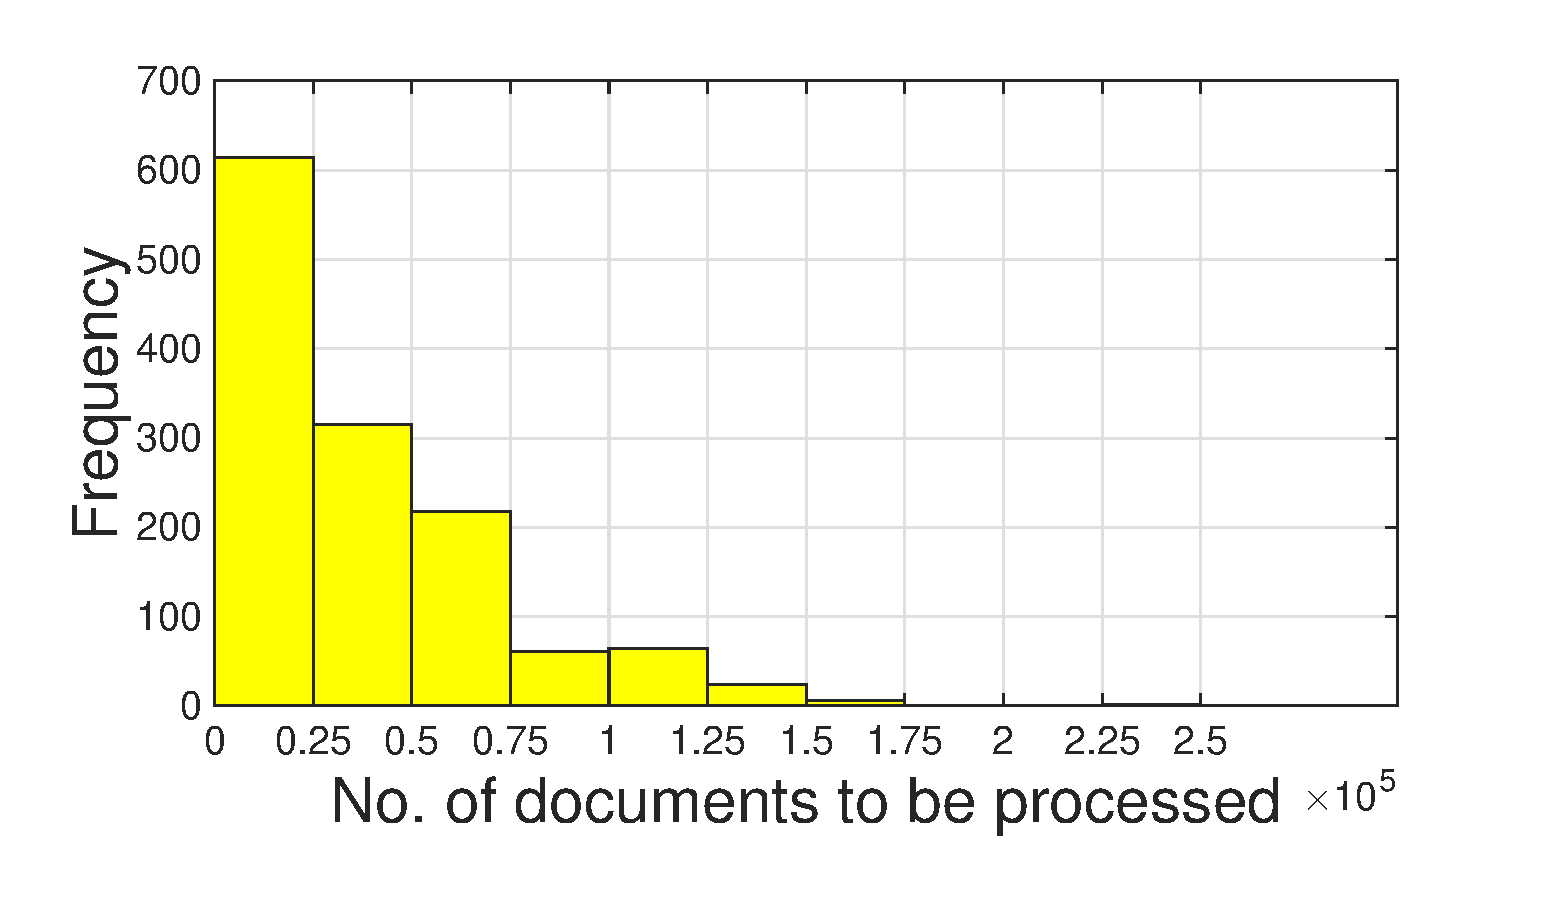
\includegraphics[width=0.70\textwidth,height=55mm]{figs/filter1}
   \caption{The distribution of the number of patents that should be ranked for each query over all test topics ($1,303$), after applying the IPC filter (filter type I).
On average, the matching process for each query is done over $ 36,254 $ documents instead of the whole collection (2.6 million documents), which dramatically reduces the computational time.}   
   \label{fig:ipcfilter-histo} 
\end{figure}
%%%%%%%%%%%%%%%%%%%%%%%%%%%%%%%%%%%%%%%%%%%%%%%%%%%%%%%%%%%%%%%%%%%%%%%%%%%%%%%%%
%\FloatBarrier 
%\noindent
Figure~\ref{fig:ipcfilter-histo} illustrates that the matching process should be only done over $25,000$ documents for the majority of queries. On average, this number is $ 36,254 $, which indicates that the system just needs to look into $ 36,254 $ documents per query on average instead of the entire collection that contains 2.6 million patent documents. Therefore, applying the IPC filter computationally saves us considerable amount of time.   

In trade off between losing 19\% of relevant patents and making the ranking process faster, we choose faster computation. In addition, we notice that the histogram falls down by increasing the number of documents that should be processed; this means that for the majority of queries the matching process is done over less number of patent documents.
%\vspace{-1cm}
%\subsubsection{Applying First two IPC code components for filtering}
%\label{subsec: Firsttwocomponents}
\paragraph{Filter Type II: Two First Components of IPC Code}
%\textbf{(B) Filter: First two components of the IPC code}
\ \\
We hypothesise that the errors will be reduced, if we broaden the filter by selecting two first components of the query IPC, namely, section, and class (e.g., C07). We repeat the experiments for filter type II.
The results have been illustrated in Figure~\ref{fig:ipc1stTwoElements}. Figure~\ref{fig:ipc1stTwoElements_a} shows that we can reduce the errors related to filtering from 19\% to 13\% by omitting the subclass component. However, the number of documents that should be ranked increases from $ 36,254 $ to $ 99,754 $ on average. As it can be seen in Figure~\ref{fig:ipc1stTwoElements_b}, the distribution of the number of documents that should be compared in matching process does not follow the falling trend as filtering with three first components. We conclude that this filter is not appropriate since we only reduce the error by 6\% whereas the average number of documents, which should be processed,~triples.    
%%%%%%%%%%%%%%%%%%%%%%%%%%%%%%%%%%%%%%%%%%%%%%%%%%%%%%%%%%%%%%%%%%%%%%%%%%%%%%%%%
%\begin{figure}[t!]
%   \centering
%   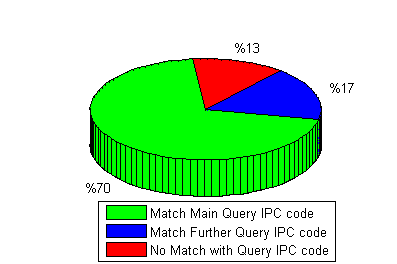
\includegraphics[width=0.55\textwidth,height=60mm]{figs/ipc1stTwoElements.png}
%   \caption{Filter: The first two components (Section and Class).}   
%   \label{fig:ipc1stTwoElements} 
%\end{figure}
%%%%%%%%%%%%%%%%%%%%%%%%%%%%%%%%%%%%%%%%%%%%%%%%%%%%%%%%%%%%%%%%%%%%%%%%%%%%%%%%%
%%%%%%%%%%%%%%%%%%%%%%%%%%%%%%%%%%%%%%%%%%%%%%%%%%%%%%%%%%%%%%
\begin{figure}[t!]
\begin{centering}
\subfigure[The portion of patents in the collection which are matched with the query IPC code. \label{fig:ipc1stTwoElements_a}]{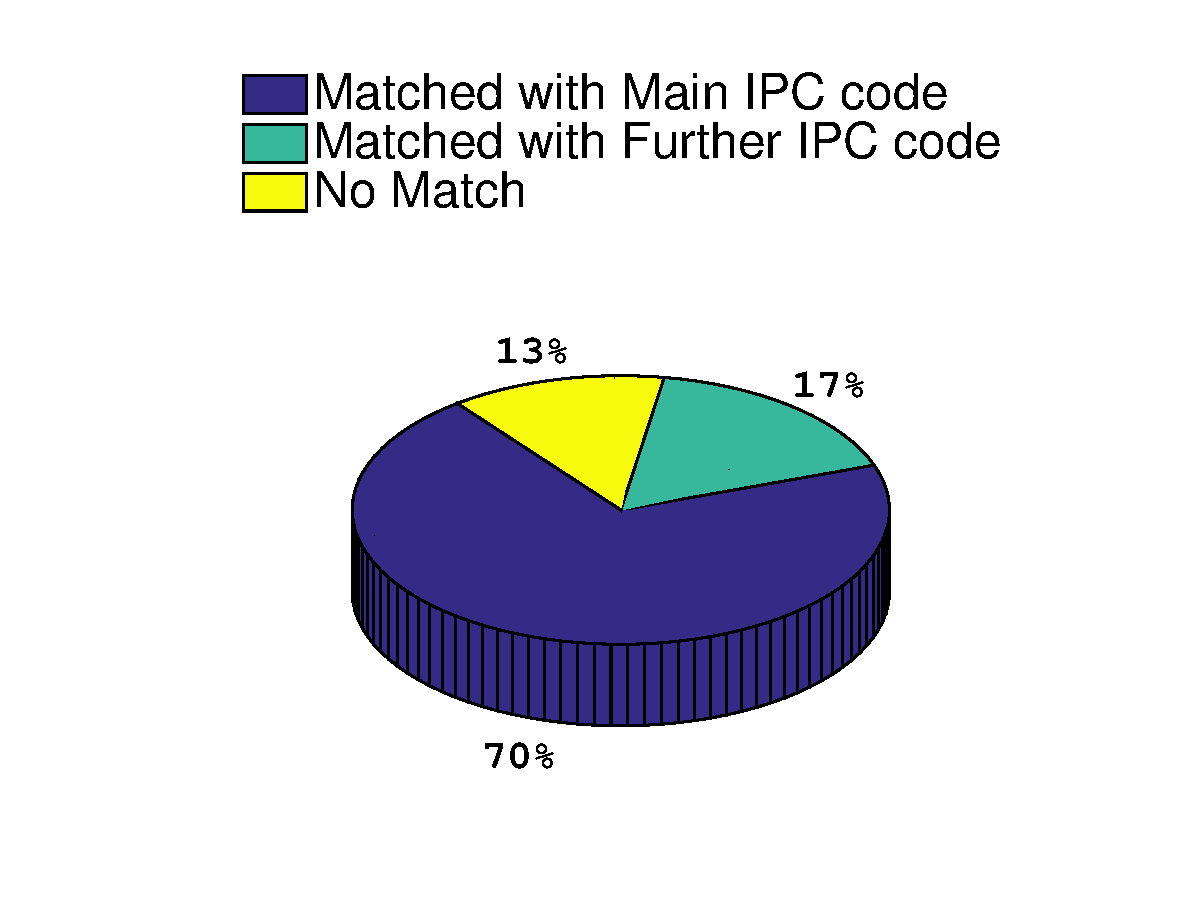
\includegraphics[width=7.5cm, height=6cm]{figs/filter2_pie}} 
\\[1ex]%
\subfigure[The distribution of the number of patents should be ranked for each query over all test queries ($1,303$).
In average, the matching process for each query is done over $ 99,754 $ documents instead of the whole collection (2.6 million documents), which dramatically reduce the computational time.\label{fig:ipc1stTwoElements_b}]{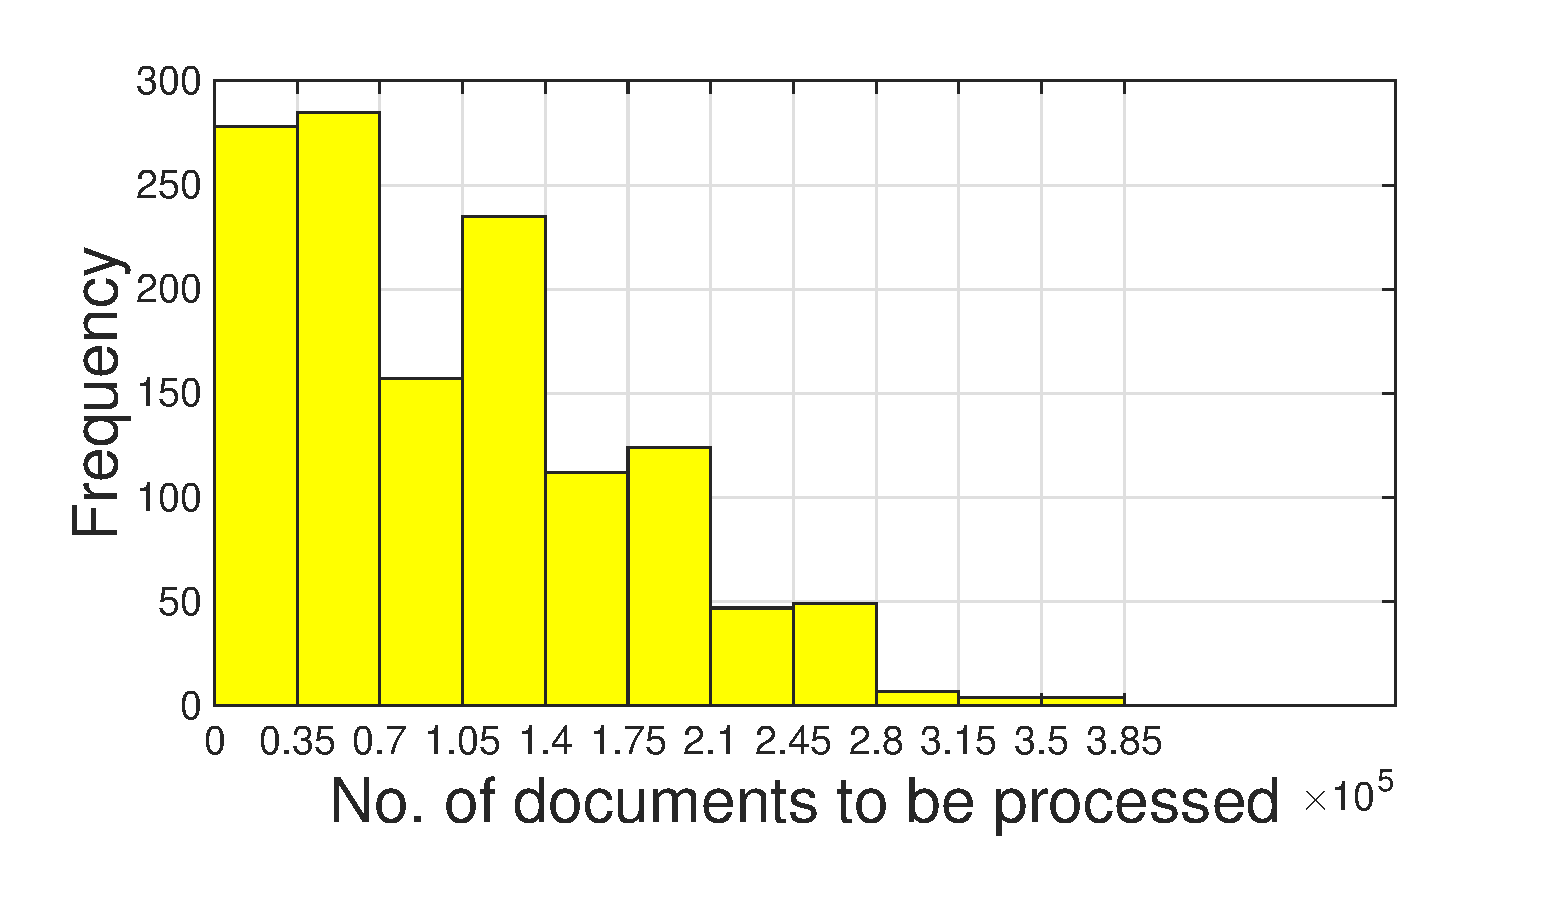
\includegraphics[width=9.5cm, height=6cm]{figs/filter2}} 

\par\end{centering} 
\protect\caption{Applying first two IPC code components (Section and Class) for filtering}
\label{fig:ipc1stTwoElements}
\end{figure}
%%%%%%%%%%%%%%%%%%%%%%%%%%%%%%%%%%%%%%%%%%%%%%%%%%%%%%%%%%%%%%
%\begin{figure}[htpb]
%\centering
%\begin{subfigure}[htpb]{.5\linewidth}
%\centering
%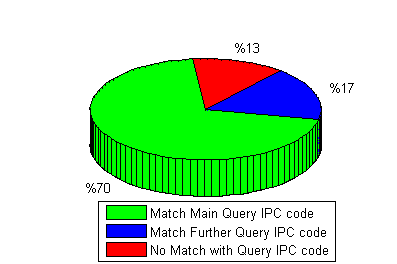
\includegraphics[width=1\textwidth,height=55mm]{figs/ipc1stTwoElements.png}
%\caption{Filter: The first two components (Section and Class)}
%\label{fig:ipc1stTwoElements}
%\end{subfigure}%\\[1ex]%
%\begin{subfigure}[htpb]{.5\linewidth}
%\centering
%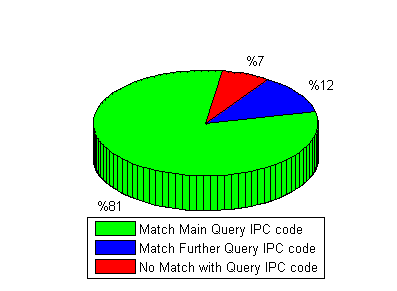
\includegraphics[width=1\textwidth,height=55mm]{figs/ipc1stElement.png}
%\caption{Filter: Only the first component (Section)}
%\label{fig:ipc1stElement}
%\end{subfigure}
%\caption{IPC classification overlap between the query and the FN patents after making the filter broader.}
%\label{fig:restrictedipc}
%\end{figure}
%\FloatBarrier
%%%%%%%%%%%%%%%%%%%%%%%%%%%%%%%%%%%%%%%%%%%%%%%%%%%%%%%%%%%%%%%%%%%%%%%%%%%%%%%%%
%\begin{figure}[t!]
%   \centering
%   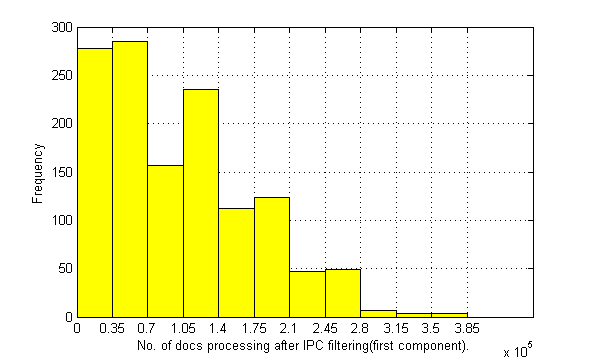
\includegraphics[width=0.70\textwidth,height=68mm]{figs/firstTwoIpcFilter-histo.png}
%   \caption{The distribution of the number of patents should be ranked for each query over all test queries (1303).
%In average, the matching process for each query is done over `$ 99754 $' documents instead of the whole collection (2.6 million documents) which reduce the computational time dramatically.}   
%   \label{fig:firstTwoIpcFilter-histo} 
%\end{figure}
%%%%%%%%%%%%%%%%%%%%%%%%%%%%%%%%%%%%%%%%%%%%%%%%%%%%%%%%%%%%%%%%%%%%%%%%%%%%%%%%%
%\FloatBarrier 
%\vspace{-5em}
%\noindent
%\subsubsection{Applying First two IPC code components for filtering}
%\label{subsec: Firsttwocomponents}
\paragraph{Filter Type III: First Component of IPC Code}
%\textbf{(C) Filter: First component of the IPC code}
\ \\
We can even make the filter more general by choosing only the first component, namely, section (e.g., C), corresponding to very general technical fields. 
%%%%%%%%%%%%%%%%%%%%%%%%%%%%%%%%%%%%%%%%%%%%%%%%%%%%%%%%%%%%%%
\begin{figure}[t!]
\begin{centering}
\subfigure[The portion of patents in the collection which are matched with the query IPC code. Filter: The first two components \label{fig:ipc1stElements_a}]{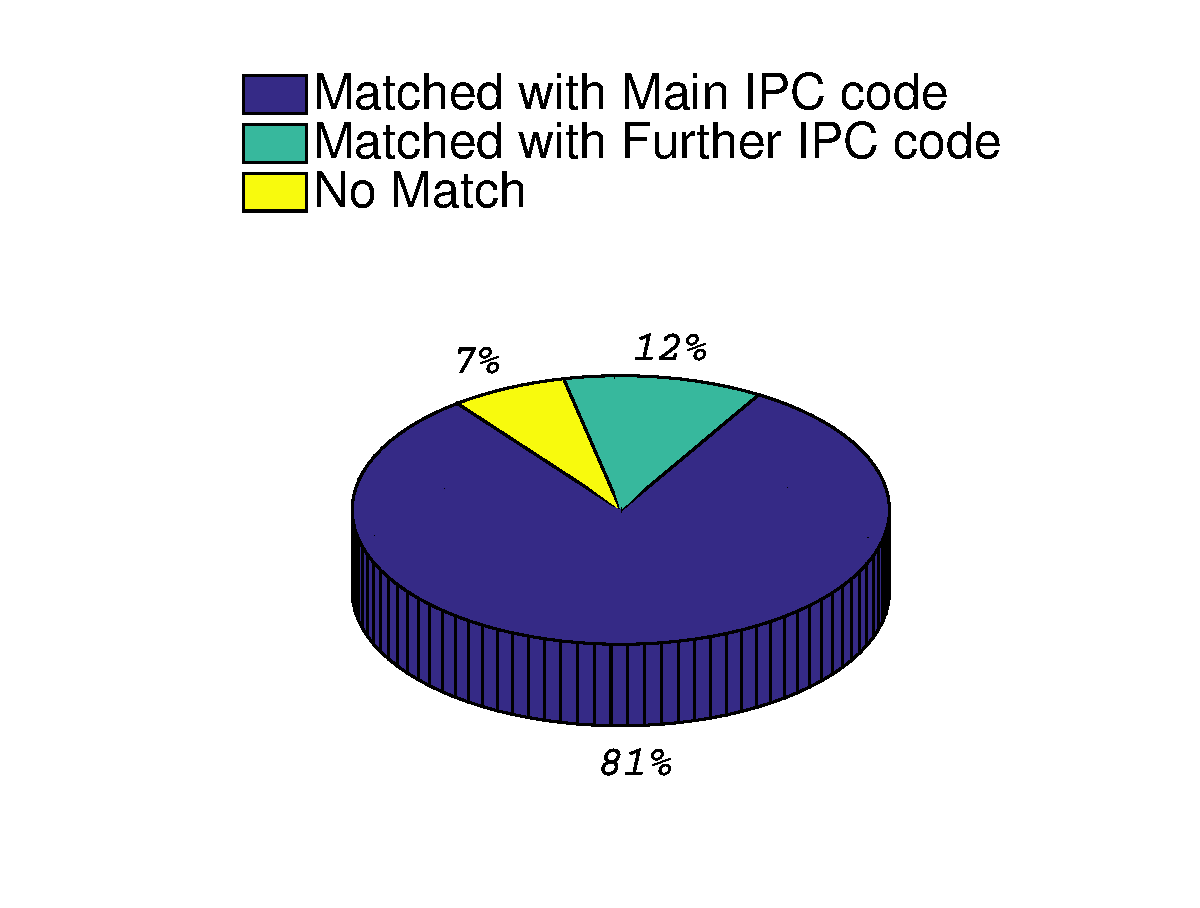
\includegraphics[width=7.5cm, height=6cm]{figs/filter3_pie}} 
\\[1ex]%
\subfigure[The distribution of the number of patents should be processed for each query after applying the IPC filter.
In average, the matching process for each query is done over $ 415,828 $ documents instead of the whole collection (2.6 million documents). This number is much higher than using more restricted filters, so it is not computationally~efficient.\label{fig:ipc1stElements_b}]{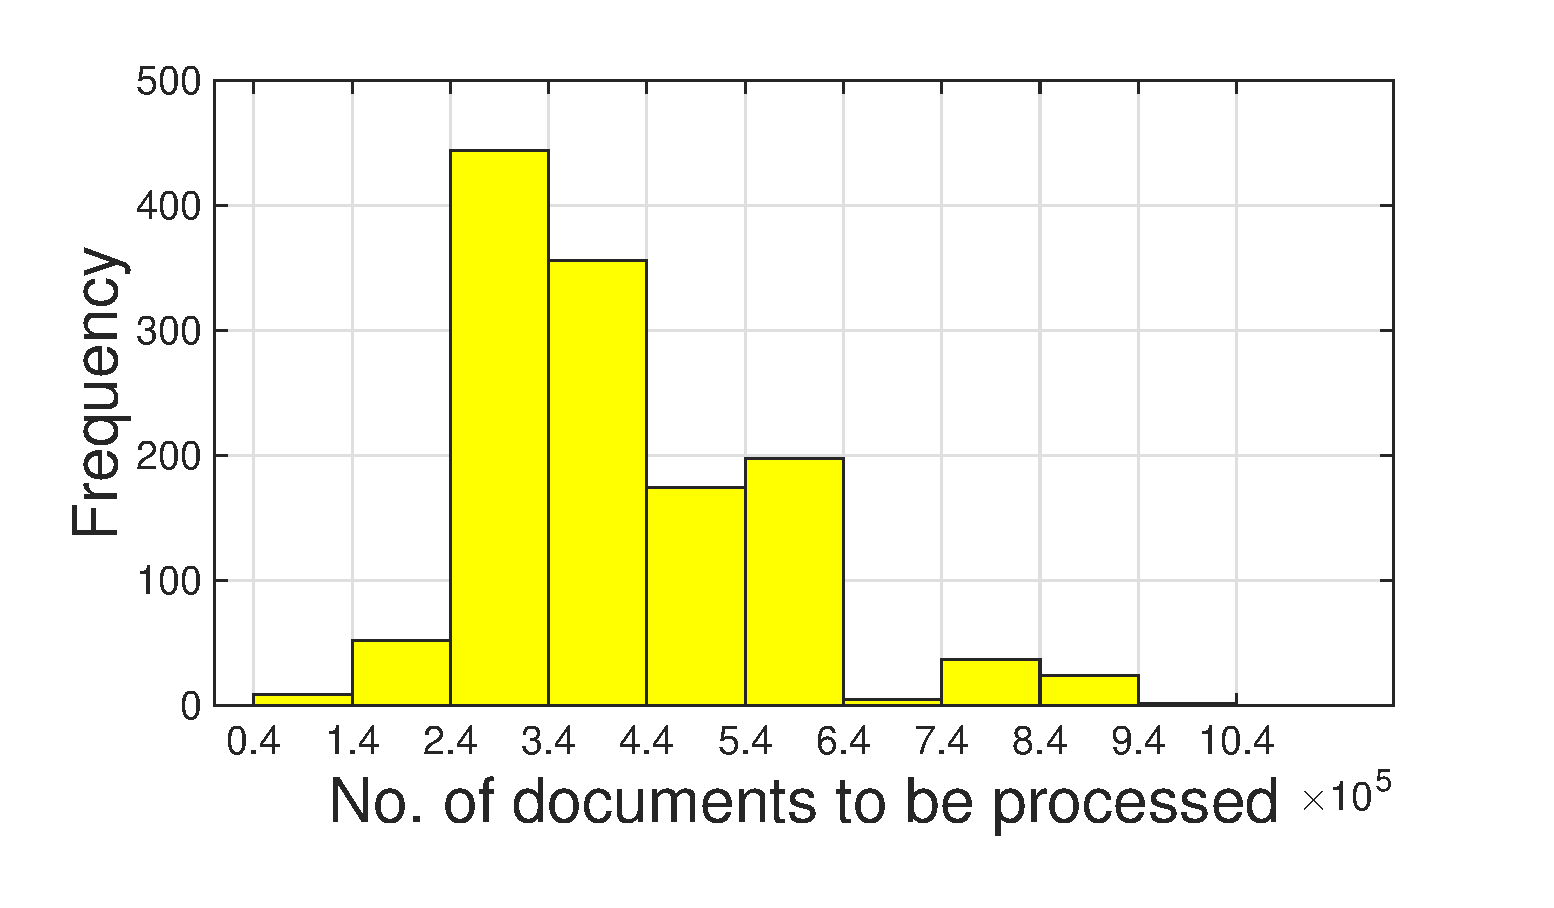
\includegraphics[width=9.5cm , height=6cm]{figs/filter3}} 

\par\end{centering} 
\protect\caption{Applying the first IPC code component for filtering (Section)}
\label{fig:ipc1stElements}
\end{figure}
%%%%%%%%%%%%%%%%%%%%%%%%%%%%%%%%%%%%%%%%%%%%%%%%%%%%%%%%%%%%%%
%%%%%%%%%%%%%%%%%%%%%%%%%%%%%%%%%%%%%%%%%%%%%%%%%%%%%%%%%%%%%%%%%%%%%%%%%%%%%%%%%
%\begin{figure}[t!]
%   \centering
%   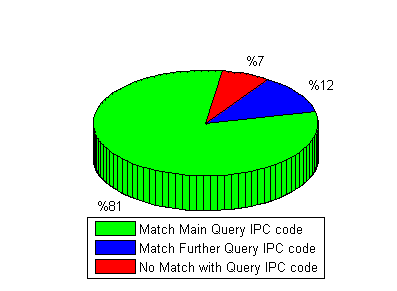
\includegraphics[width=0.50\textwidth,height=55mm]{figs/ipc1stElement.png}
%   \caption{Filter: Only the first component (Section).}   
%   \label{fig:ipc1stElements} 
%\end{figure}
%%%%%%%%%%%%%%%%%%%%%%%%%%%%%%%%%%%%%%%%%%%%%%%%%%%%%%%%%%%%%%%%%%%%%%%%%%%%%%%%%
Figure~\ref{fig:ipc1stElements_a} shows that about 7\% of relevant patents do not share the most general component of the query IPC Code. 
Figure~\ref{fig:ipc1stElements_b} shows the distribution of the number of patents should be ranked for each query after applying the IPC filter.
%: ``\textit{only the first component of the IPC code}". 
The results show that the matching process for each query is done over $ 415,828 $ documents, on average, instead of the whole collection (2.6 million documents). This number is much higher than the number for previous filters, which shows that using only the first component of the IPC code is not computationally efficient because it does not reduce the computational time as well as it still causes 7\% of the errors. 
%The min number of documents considered during matching process is `$ min=41721 $', and the maximum is `$ max=1058447 $'. 
%\vspace{-2em}
%%%%%%%%%%%%%%%%%%%%%%%%%%%%%%%%%%%%%%%%%%%%%%%%%%%%%%%%%%%%%%%%%%%%%%%%%%%%%%%%%
%\begin{figure}[t!]
%   \centering
%   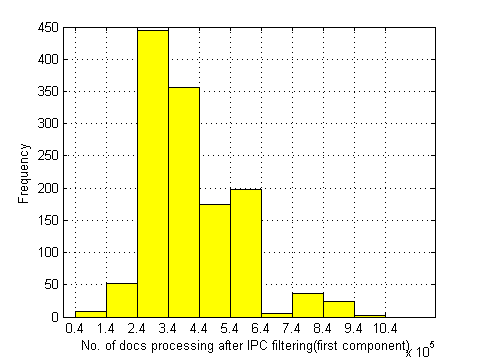
\includegraphics[width=0.60\textwidth,height=60mm]{figs/firstIpcFilter-histo.png}
%   \caption{The distribution of the number of patents should be ranked for a query over all test queries (1303), after applying the IPC filter: ``\textit{only the first component of the IPC code}".
%In average, the matching process for each query is done over `$ 415828 $' documents instead of the whole collection (2.6 million documents). This number is much higher than using more restricted filters and will not be efficient computationally. 
%%The min number of documents considered during matching process is `$ min=41721 $', and the maximum is `$ max=1058447 $'
%}   
%   \label{fig:firstIpcFilter-histo} 
%\end{figure}
%%%%%%%%%%%%%%%%%%%%%%%%%%%%%%%%%%%%%%%%%%%%%%%%%%%%%%%%%%%%%%%%%%%%%%%%%%%%%%%%%

To recap our experiments related to the IPC code filtering, we showed that, in trade off between the errors related to applying IPC code filter and computationally efficient matching process, we got the best results when we applied the first three IPC code (section, class, and subclass) of the reference query as a filter. The filter reduced the number of documents to be ranked from the whole collection to $ 36,254 $ documents on average, so using the IPC filter saved a considerable amount of computational time.
%%%%%%%%%%%%%%%%%%%%%%%%%%%%%%%%%%%%%%%%%%%%%%%%%%%%%%%%%%%%%%%%
%%%%%%%%%%%%%%%%%%%%%%%%%% Section 4 %%%%%%%%%%%%%%%%%%%%%%%%%%%
%%%%%%%%%%%%%%%%%%%%%%%%%%%%%%%%%%%%%%%%%%%%%%%%%%%%%%%%%%%%%%%%
%\section{New Evaluation: Excluding Identified Errors}
{
%\scriptsize
%\sffamily
\ttfamily\small
 \begin{tabular}{lcc}
 \hline\noalign{\smallskip} 
  & \multicolumn{1}{p{3cm}}{\centering Patent Query \\Not-Filtered} &\multicolumn{1}{p{3cm}}{\centering Patent Query \\Filtered} \\ 
 \noalign{\smallskip} 
\hline 
\noalign{\smallskip} 
\vtop{\hbox{\strut PRES}\hbox{\strut MAP}\hbox{\strut A. Recall}} 
& \vtop{\hbox{\strut 0.3910}\hbox{\strut 0.1214}\hbox{\strut 0.4008}}
& \vtop{\hbox{\strut 0.5355}\hbox{\strut 0.1618}\hbox{\strut 0.5491}} \\

\hline 
 \end{tabular} 
 
}
%%% Local Variables: 
%%% mode: latex
%%% TeX-master: t
%%% End: 
%%%%%%%%%%%%%%%%%%%%%%%%%%%%%%%%%%%%%%%%%%%%%%%%%%%%%%%%%%%%%%%%
%%%%%%%%%%%%%%%%%%%%%%%%%% Section 4 %%%%%%%%%%%%%%%%%%%%%%%%%%%
%%%%%%%%%%%%%%%%%%%%%%%%%%%%%%%%%%%%%%%%%%%%%%%%%%%%%%%%%%%%%%%%
%\section{Summary}
%\label{sce: summary3}
%We developed a baseline IR system for patent prior art search on the top of
the Lucene search engine\footnote{\texttt{http://lucene.apache.org/}}, which processes queries using both BM25~\cite{Robertson1993} and LM (Dirichlet
smoothing, and Jelinek-Mercer smoothing)~\cite{zhai2004study} scoring functions. %We consider 
%using BM25F~\cite{robertson2004simple} but had no opportunity to learn appropriate field weights.
We used Lucene to index the English subset of CLEF-IP 2010 dataset\footnote{\texttt{http://www.ifs.tuwien.ac.at/\textasciitilde{}clef-ip/}} 
(Section~\ref{sec:DataCollection}) that contains 2.6 million patent documents and 1303 topics (queries) for the English test set.
We used the default Lucene settings using the Porter stemming algorithm \cite{Porter1980} and English stop-word removal. 
We also removed patent-specific stop-words as described in \cite{magdy2012toward}.
In
our implementation, each section of a patent (title, abstract, claims,
and description) is indexed in a separate field. However, when a query 
is processed, all indexed fields are targeted with an equal weight, since this generally
offers best retrieval performance. We also used the International
Patent Classification (IPC) codes assigned to the topics to filter
the search results by constraining them to have common IPC codes with
the patent topic as suggested in previous works~\cite{lopez2010patatras}.
Although this IPC code filter may prevent retrieval of relevant patents, we
have chosen to keep it for the following reasons: (i) more than 80\%
of the patent queries share an IPC code with their associated relevant
patents, and (ii) it makes the retrieval process much faster. The accuracy of the results is evaluated using two popular metrics --- Mean Average Precision (MAP) and Average Recall --- on the top-100 results for each query, assuming that patent examiners are willing to assess the top 100 patents \cite{joho2010survey}. 
We achieved the best performance while querying with the Description
section as in previous work \cite{xue2009transforming} and using
either the LM or the BM25 scoring functions. We call this initial
query the \textit{Patent Query} and use it as our main baseline.

In addition, we compare our results to \textit{PATATRAS}, a highly engineered system developed by Lopez and Romary~\cite{lopez2010experiments}, which achieved the best performance in the CLEF-IP 2010 competition. This system uses multiple retrieval models (especially Kullback-Leibler divergence~\cite{Baeza-Yates2011} and Okapi BM25) and exploits patent metadata and citation structures.  While our evaluation excludes 22 of the 1303 topics for which no relevant English documents were available, the difference in MAP score between our evaluation and the full 1303 topic evaluation of PATATRAS is negligible. We exclude 22 queries because the focus of our research has been on term analysis and errors related to term matching process of ranking functions. So, we eliminated data curation errors and IPC filter errors--- as they will be described in Section~\ref{sec:DataCurationErrors} and Section~\ref{sec:ClassificationCodeMismatch}--- to increase the accuracy of our data analysis results. 
%did not include errors related to non-English patents in our evaluation and we mainly focus on errors related to term matching for English patents.  
%However, the MAP we provide is not directly comparable since we excluded 22 topics from our evaluation because their relevant patents were not in English or had no IPC code matched with the topic. We pruned these topics out because we were only interested in analysing errors related to term matching. Removing 22 topics caused only 0.04 improvement in our baseline system, which is negligible. Hence, we use Top CLEF-IP 2010 results for a rough comprasion."}
% 

% TODO: Don't exclude 22 topics!





\section{Oracular Term Selection}
\label{Sec:OracularTermSelection}
% What does this text have to do with the oracular query that this
% section introduces???  You have to explain the most salient features
% of the section -- like the title -- before diving into details!  -Scott
%
% The main complaint about patent search is an
% insufficient match between the content of patent queries and
% relevant
% patents\cite{lupu2013patent}\cite{magdy2012toward}. However,
% considering the size of a patent query (usually thousand of words),
% the intuition is that there are enough terms to match the relevant
% patents.

In this section we develop an \emph{Oracular Query} to understand (a)
the adequacy of the baseline
\emph{Patent Query}, (b) an upper bound on performance of the
BM25 and LM models, and (c) the sufficiency of terms in the reference
patent query.

\subsection{Oracular Query Formulation}

% As noted previously, I would be careful calling this ``relevance feedback''
% and especially abbreviating it RF since RF usually has a different definition
% based on a vector space or other model.  I would call it AvgRelDiff or
% something similar.  -Scott
We begin by defining an oracular relevance feedback system, which
extracts terms from the judged relevant documents.  To this end, after an initial run of a given query, we
calculate a Relevance Feedback ($\mathit{RF}$) score for each term in the top-100
retrieved documents as follows:
% Use \mathit{RF}, \mathit{Rel}, etc. for multiletter names, 
% otherwise RF is technically R*F!  Fix.  -Scott
\begin{equation}
RF(t,Q)=Rel(t)-Irr(t) 
 \label{eq:score}
\end{equation}\vspace*{-5ex}
\begin{displaymath}t\in \lbrace \mbox{terms in top-100 retrieved documents}\rbrace\end{displaymath}
where $ \mathit{Rel(t)} $ is the average term frequency in retrieved relevant patents and $ \mathit{Irr(t)} $ is the average term frequency in retrieved irrelevant patents. We assume that words with a positive score are \emph{useful words} since they are more frequent in relevant patents, while words with negative score are \emph{noisy words} as they appear more frequently in irrelevant patents. We empirically seek to evaluate the threshold $\tau$ on $RF(t,Q)$ (defined below) yielding the best oracular query.

%that determines if a term is selected to build the \emph{Oracular Query} or not.

% Huh??? -Scott
%
%We expected to see a higher performance for the queries which contain more \textit{ useful words}, but, surprisingly, we could not find any correlation between the performance and the presence of \textit{ useful words} in the query. 

%We hypothesized that a query, formulated by only the \textit{ useful terms}, is the best possible query we can make since they are all frequent in relevant patents but rare in irrelevant ones. 
We formulate two oracular queries. The first query is formulated by selecting terms in the top-100 documents:
\begin{equation}
Oracular \; Query = \{t \in top-100|RF(t, Q)>\tau\}   
 \label{eq:score}
\end{equation}
We formulate the second query by selecting terms that also occur in the reference patent query as follows:
% query based on the hypothesis that a patent query contains sufficient words matched with the relevant patents:
\begin{equation}
 Oracular \; Patent \; Query = \{t\in Q|RF(t, Q)>\tau\}   
 \label{eq:score}
\end{equation}
%The system performance to these two queries were encouraging. We discuss the detailed results in the next section.

\subsection{Baseline vs. Oracular Query}

\label{sec:baseline_vs_oracular}

%%%%%%%%%%%%%%%%%%%%%%%%%%%%%%%%%%%%%%%%%%%%%%%%%%%%%%%%%%%%%%
\begin{figure}[t!]
\begin{centering}
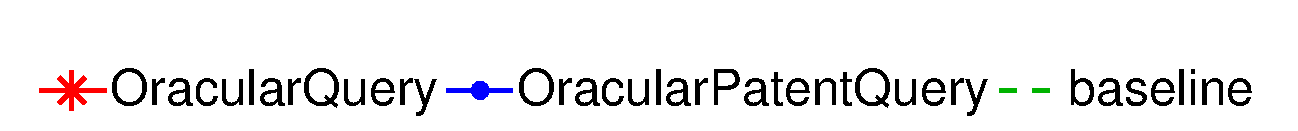
\includegraphics[width=9cm]{imgs/l1}
\par\end{centering}

\begin{centering}
\subfigure[{Mean Average Precision.}]{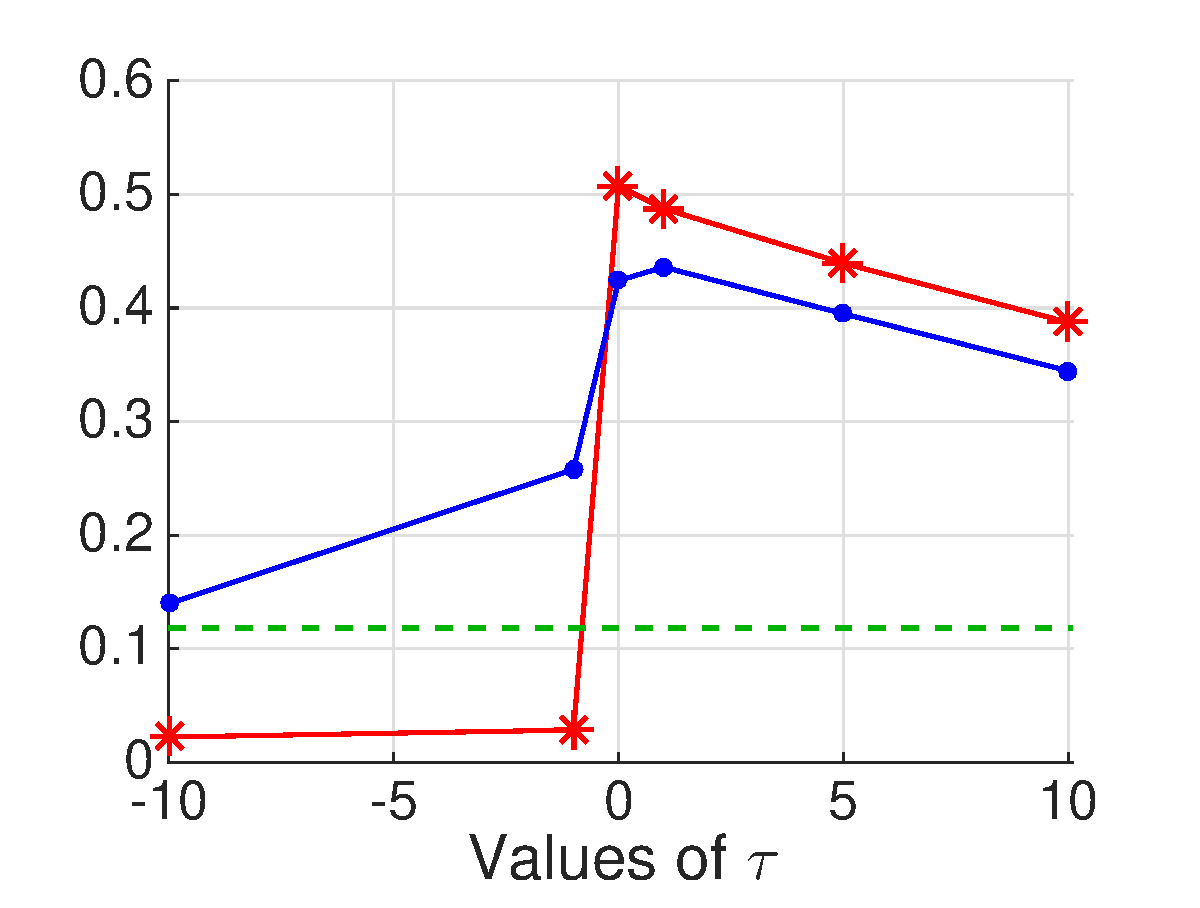
\includegraphics[width=4.5cm]{imgs/fig1_map}}\subfigure[Recall.]{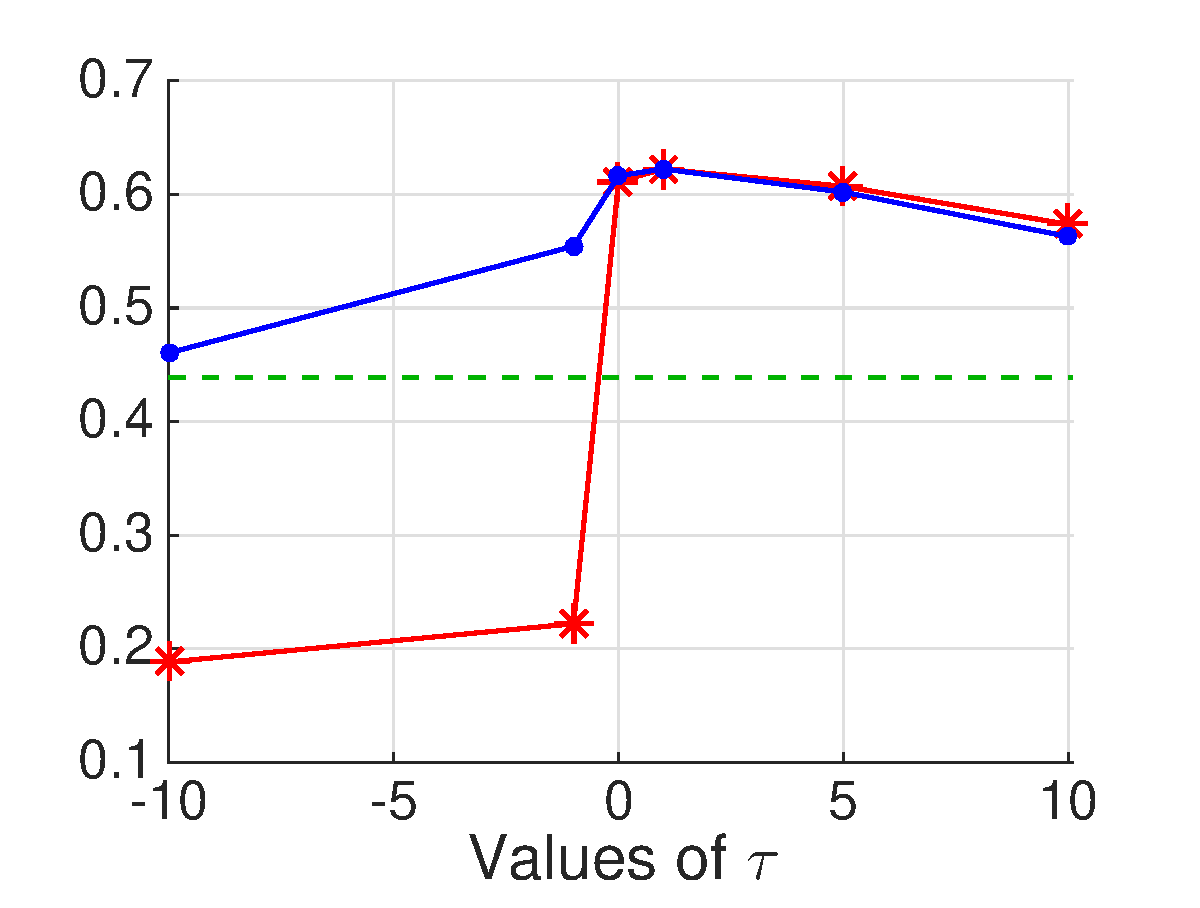
\includegraphics[width=4.5cm]{imgs/fig1_recall}}
\par\end{centering}

\protect\caption{System performance vs. the threshold $\tau$ for Oracular Query and Oracular Patent Query.}
\label{fig:oracular}
\end{figure}
%%%%%%%%%%%%%%%%%%%%%%%%%%%%%%%%%%%%%%%%%%%%%%%%%%%%%%%%%%%%%%

First, we investigate the ideal threshold setting $\tau$.
%\in\{-10,$ $-5,0,5,10\}$.
Figure \ref{fig:oracular} illustrates that $\tau=0$ is the
best-performing value for \emph{Oracular Query} while $\tau=1$ is the
best for \emph{Oracular Patent Query}. In general, the MAP and the recall for the \emph{Oracular
Patent Query} are lower than the MAP and the recall for the \emph{Oracular Query} respectively;
nonetheless the terms selected from the reference patent query itself are
still sufficient to achieve MAP performance significantly better than the PATATRAS system. In addition, we remark on the rather
unexpected steep drop-off in performance when the oracular query
includes slightly noisy terms (i.e., $\tau$ just slightly less than 0)
as defined previously.

% What is the ``Best Run''???  You cannot make up words and expect the
% reader to understand.  Be precise on the first introduction that
% this is the best result from CLEF-IP 2010 and provide a citation.
% And call it the ``Top CLEF-IP 2010'' system to be crystal clear.
% Furthermore, it has been mentioned previously that the MAP from CLEF-IP 2010
% and the MAP you provide are not directly comparable since some topics are
% excluded from this evaluation --- for full disclosure you need to explain
% all details of how these MAP measurements differ (and hence indicate this
% Top CLEF-IP 2010 result is only included for a rough comparison of
% performance).  Fix all of these issues and all name changes resulting
% from these updates.  -Scott
%
% Update this discussion with the new table contents.  -Scott
%
% Also, streamline the text... so many sentences are redundant or 
% unneccessary!  You're not done writing until you've removed every
% word possible without changing the meaning of what's written.  -Scott
%
% If different \tau's were used then be clear on this, or simply mention
% Oracular Patent Query $\tau=1$ in the table entry and mention in the
% text how this optimal \tau was selected.  Maybe Figure 1 should come
% before Table 1?  This would better explain how the best \tau's were
% selected.  -Scott
%

%%%%%%%%%%%%%%%%%%%%%%%%%%%%%%%%%%%%%%%%%%%%%%%%%%%%%%%%%%%%%%
\begin{table}[t!]
  \begin{center}
  \scriptsize
   \caption{Performance for the \textit{ Patent Query}, two variants of the \textit{ Oracular Query}, and \textit{ Top CLEF-IP 2010 (PATATRAS)}.}
   \vspace*{1ex}
  \input table/optquery.tex   
  \label{tab:optquery}
  \end{center}  
\end{table}
%%%%%%%%%%%%%%%%%%%%%%%%%%%%%%%%%%%%%%%%%%%%%%%%%%%%%%%%%%%%%%

In Table~\ref{tab:optquery}, we compare our two oracular relevance
queries with both the baseline \textit{Patent Query} and the PATATRAS system.  Here we see that
the \emph{Oracular Query} using $\tau=0$ far outperforms the baseline and
approximately performs twice as well on MAP as the PATATRAS system, the best competitor in
CLEF-IP 2010. 
%Roughly 50\% improvement for the recall is achieved with respect to the baseline \textit{Patent Query}. 
In general we found BM25 and LM to offer very similar performance.  Our subsequent results use only LM due to space limitations although results for BM25 are very similar.
%
% Unweighted is most natural so no need to even mention it.  -Scott
%
%We observed that a weighed --by query term
%frequency-- query performs better than the unweighed one. However, our
%oracular query performed better unweighed, so, we compare the results
%with unweighed baseline query. The \textit{ best run} in CLEF-IP 2010
%achieved 0.27 MAP~\cite{lopez2010experiments}.

%Next, we used a threshold $\tau$ to formulate the \textit{ Oracular Query}
%and \textit{ Oracular Patent Query} to include merely terms with the RF
%score higher than $\tau$ ($RF(t,Q)>0$).

% Good: is space allows, the enumeration helps make the take-home points
% of this section clear for the reader and leads into the next section.  -Scott
Overall, our experiments related to oracular relevance feedback system
suggest two important conclusions: (1) query reduction should suffice for effective prior art patent retrieval; and (2) very precise methods for eliminating poor query terms in the reduction process are needed.




\section{Query Reduction: Approximating the Oracular Query}
\label{Sec:QueryReduction}
The gain achieved using the Oracular Patent Query method motivated us to explore various methods to approximate the terms
selected by this query without ``peeking at the answers'' provided by
the actual relevance judgements.  We first attempt this via fully
automated methods and then proceed to evaluate semi-automated methods
based on interactive relevance feedback methods.

\subsection{Automated Reduction}
\label{sec:AutomatedReduction}
%\vspace*{-2ex}
%We noticed that most of the useful feedback terms exist in the original query and hypothesized that the baseline system could be substantially improved by removing negative query terms. 
%
% Why these approaches? provide citations for who has suggested them or otherwise
% provide a justification as to why each approach would be a good idea.  Do this
% in the bullet points where the actual method is discussed... not after the bullet
% points!  Don't dissociate content and discuss it multiple times in different
% places!  -Scott
We use the following four simple approaches to reduce the initial patent queries: 
%(i) removing Document Frequent terms (IDF(t)>$\tau$), (ii) keeping Frequent Terms in Query (QTF(t)>$\tau$); (iii) using Pseudo Relevance Feedback set (constructed after an initial run of the query) to select query terms (PRF(t)>$\tau$); and (iv) removing general terms in IPC title. 

\vspace*{0.5mm}
\noindent \textbf{(1)} In standard IR approaches, removing terms, appearing a lot in the collection, helps the retrieval effectiveness. Inspired by this fact, after an initial run of the query, we removed terms  with a high average term frequency over the top-100 documents ($DF(t)>\tau$). However, as illustrated in Figure \ref{fig:queryreduc}, this technique significantly hurts the performance.  

\vspace*{0.5mm}
\noindent \textbf{(2)} Intuitively, frequent terms inside long and verbose queries are  important~\cite{maxwell2013compact}. Hence, we only kept frequent terms inside the query ($QTF(t)>\tau$).  Figure \ref{fig:queryreduc} indicates that this approach perform just slightly over the baseline.

\vspace*{0.5mm}
\noindent \textbf{(3)} The third approach to reduce query is query term selection using Pseudo Relevance Feedback ($\mathit{PRF}$)~\cite{Baeza-Yates2011, maxwell2013compact}. We calculated a $\mathit{PRF}$ score similar to $\mathit{RF}$ score assuming the top k ranked documents are relevant. As it can be seen in Figure \ref{fig:queryreduc}, this approach do not also, notably, outperform the baseline. 
%In fact, we could not find any heuristic correlation between  $ PRF(t)$ and $ RF(t)$. 

\vspace*{0.5mm}
\noindent \textbf{(4)} Finally, we used words in IPC code title of each patent query to reduce the query, based on the assumption that they are common to all patents, which belong to the same category and may be considered as stop-words. In our experiment, we removed the IPC title terms from a selection of frequent query terms ($QTF(t)>5$). We can see in Figure \ref{fig:queryreduc} that the results drop slightly compared to the approach 2, where $\tau=5$.
%\noindent \textbf{(1)-} In standard IR approaches, removing terms, appearing a lot in the collection, helps the retrieval effectiveness. Inspired by this fact, after an initial run of the query, we removed terms  with a Document Frequency (DF) in top-100 documents, higher than the threshold $\tau$. However, as illustrated in Figure \ref{fig:queryreduc}, it's clear that this technique significantly hurts the performance ($DF(t)>\tau$).  
%
%\noindent \textbf{(2)-} Intuitivelly, frequent terms inside long and verbose queries are  important~\cite{maxwell2013compact}. Hence, we have  choosen to reduce queries by selecting terms with a frequency higher than a certain threshold $\tau$. The results in Figure \ref{fig:queryreduc} indicate clearly that this simple and naive technique is not adequate ($QTF(t)>\tau$). 
%
%\noindent \textbf{(3)-} The third approach we experiment to reduce the query is based on Pseudo Relevance Feedback ($\mathit{PRF}$)~\cite{Baeza-Yates2011}. $\mathit{PRF}$ is an automated process without user interaction, which assumes the top k ranked documents are relevant. Again, it can be seen in Figure \ref{fig:queryreduc} that the results for query reduction using $\mathit{PRF}$ do not notably outperform the baseline. In fact, we could not find any heuristic correlation between  $ PRF(t)$ and $ RF(t)$. 
%%Reda: Need clearly to be explained!}
%
%\noindent \textbf{(4)-} Finally, we used words in IPC code title of each patent query to reduce the query, based on the assumption that they are common to all patents, which belong to the same category and may be considered as stop-words. However it did not help.

%we hurt the effectiveness by filtering them out.

% The anecdotal results and their implications have to be explained
% much more clearly... what is surprising about them (be specific:
% point out actual terms) and what can you take away from this
% investigation.  -Scott
\vspace*{0.5mm}
Figure \ref{fig:anecdotal} shows an anecdotal example for a sample query about an invention related to ``emulsifier'', to explain why these four approaches fail. It shows the raw abstract of the invention, and terms and their associated associated $\mathit{RF}$ scores for each category. Terms are chosen as follows: $\{t| DF(t)/QTF(t)/PRF(t)>10\} $. It can be seen that the four methods fail clearly to discriminate between useful and noisy terms. As an example, terms like ``emulsifier'', ``enzym'' and ``starch'' have been removed by the first method, which leads in decreasing the quality of the query. As for the last method, it contains more noisy terms than useful terms (19 out of 32, and few of them with high negative score like ``saccharid'' or ``amylos''), but there are still some positive terms which we remove from the reference query that can harm the query reduction method.
%which resulted in bad retrieval performance. 
%Therefore, this may suggest more sophisticated query reduction methods, as the one discussed in the next section.
 

%high scored terms are polluted with the sufficient amount of noise to hurt the retrieval effectiveness. Unfortunately, none of the proposed query reduction approaches for query reduction worked better than the baseline, which leads us to investigate interactive methods for reduction in the next section.

\subsection{Semi-automated Interactive Reduction}

\label{sec:SemiAutomatedInteractiveReduction}

%%%%%%%%%%%%%%%%%%%%%%%%%%%%%%%%%%%%%%%%%%%%%%%%%%%%%%%%%%%%
\begin{figure}[t!]
\begin{centering}
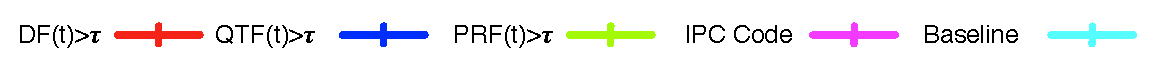
\includegraphics[width=9cm]{imgs/legend2}
\par\end{centering}

\begin{centering}
\subfigure[{Mean Average Precision.}]{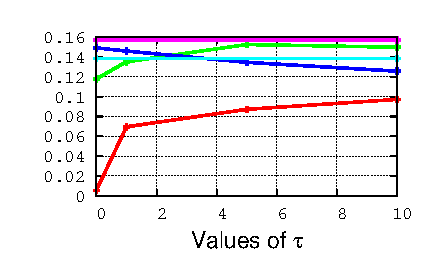
\includegraphics[width=4.5cm]{imgs/figure2-MAP}}\subfigure[Recall.]{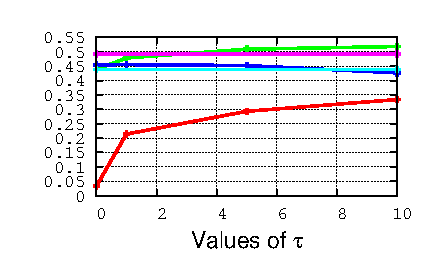
\includegraphics[width=4.5cm]{imgs/figure2-Recall}}
\par\end{centering}

\protect\caption{System performance vs. the threshold $\tau$ for four query reduction approaches.}
\label{fig:queryreduc}
\end{figure}
%%%%%%%%%%%%%%%%%%%%%%%%%%%%%%%%%%%%%%%%%%%%%%%%%%%%%%%%%%%%

%%%%%%%%%%%%%%%%%%%%%%%%%%%%%%%%%%%%%%%%%%%%%%%%%%%%%%%%%%%%
\begin{figure}[t!]
\begin{framed}
\vspace*{-2ex}
  \centering
    %\lstinputlisting[frame=single, basicstyle=\scriptsize\ttfamily , linewidth=\columnwidth,breaklines=true]{code/anecdotale.tex}\vspace*{-2ex}
 \begin{lstlisting}[basicstyle=\scriptsize\ttfamily , linewidth=\columnwidth,breaklines=true] 
PAC-1293
Abstract: The invention relates to an emulsifier, 
a method for preparing said emulsifier, and to 
its use in various applications, primarily food 
and cosmetic applications. The invention also 
relates to the use of said emulsifier for the 
creation of an elastic, gelled foam. An 
emulsifier according to the invention is based on 
a starch which is enzymatically converted, using 
a specific type of enzyme, and modified in a 
specific esterification reaction.

DF Terms: <@\textcolor{blue}{starch:14.64}@>, <@\textcolor{blue}{enzym:29.49}@>, <@\textcolor{red}{amylos:-20.15}@>, 
<@\textcolor{blue}{oil:8.63}@>, <@\textcolor{red}{dispers:-8.66}@>, <@\textcolor{red}{ph:-4.55}@>, <@\textcolor{red}{dry:-6.21}@>, <@\textcolor{red}{heat:-2.26}@>, 
<@\textcolor{red}{product:-5.48}@>, <@\textcolor{red}{slurri:-11.48}@>, <@\textcolor{blue}{viscos:7.77}@>, <@\textcolor{red}{composit:-4.49}@>, 
<@\textcolor{red}{reaction:-1.97}@>, <@\textcolor{red}{food:-11.94}@>, <@\textcolor{blue}{agent:5.19}@>, <@\textcolor{red}{debranch:-10.58}@>, 
<@\textcolor{red}{reduc:-6.37}@>, <@\textcolor{red}{fat:-12.83}@>, <@\textcolor{red}{prepar:-0.82}@>, <@\textcolor{red}{hour:-5.42}@>, 
<@\textcolor{blue}{waxi:19.41}@>, <@\textcolor{blue}{deriv:11.97}@>, <@\textcolor{red}{content:-3.38}@>, <@\textcolor{blue}{aqueou:0.38}@>, 
<@\textcolor{red}{saccharid:-11.95}@>, <@\textcolor{red}{ml:-0.79}@>, <@\textcolor{red}{cook:-10.04}@>, <@\textcolor{blue}{modifi:5.65}@>, 
<@\textcolor{blue}{solid:5.50}@>, <@\textcolor{blue}{sampl:6.27}@>, <@\textcolor{blue}{mix:2.48}@>, <@\textcolor{red}{minut:-1.68}@>, <@\textcolor{red}{dri:-0.91}@>, 
<@\textcolor{red}{gel:-9.85}@>, <@\textcolor{blue}{activ:5.98}@>, <@\textcolor{red}{corn:-5.27}@>, <@\textcolor{blue}{alpha:12}@>, <@\textcolor{red}{sprai:-2.74}@> 

QTF Terms: <@\textcolor{blue}{starch:14.64}@>, <@\textcolor{blue}{emulsifi:6.72}@>, <@\textcolor{red}{succin:-3.46}@>, 
<@\textcolor{blue}{enzym:29.49}@>, <@\textcolor{blue}{emuls:12.66}@>, <@\textcolor{blue}{hydrophob:5.45}@>, <@\textcolor{red}{anhydrid:-5.47}@>, 
<@\textcolor{red}{reaction:-1.97}@>, <@\textcolor{red}{octenyl:-0.66}@>, <@\textcolor{blue}{stabil:3.64}@>, <@\textcolor{blue}{alkenyl:0.06}@>, 
<@\textcolor{blue}{reagent:1.17}@>, <@\textcolor{blue}{carbon:0.12}@>, <@\textcolor{blue}{potato:3.74}@>, <@\textcolor{red}{alkyl:-0.33}@>, 
<@\textcolor{red}{wt:-4.57}@>, <@\textcolor{blue}{ether:1.96}@>, <@\textcolor{red}{enzymat:-3.45}@>, <@\textcolor{blue}{convers:10.44}@>, 
<@\textcolor{red}{chain:-5.53}@>, <@\textcolor{blue}{atom:0.03}@>, <@\textcolor{red}{ph:-4.55}@>, <@\textcolor{red}{treat:-0.89}@>, 
<@\textcolor{red}{ammonium:-1.96}@>, <@\textcolor{red}{food:-11.94}@>, <@\textcolor{red}{amylos:-20.15}@>, 
<@\textcolor{red}{glucanotransferas:-0.86}@>, <@\textcolor{red}{glycidyl:-0.40}@>, <@\textcolor{red}{glycosyl:-0.02}@>, 
<@\textcolor{red}{dry:-6.21}@>, <@\textcolor{blue}{deriv:11.97}@>, <@\textcolor{blue}{transferas:0.89}@>, <@\textcolor{red}{foam:-0.49}@>, 

PRF Terms: <@\textcolor{blue}{starch:14.64}@>, <@\textcolor{blue}{encapsul:17.50}@>, <@\textcolor{red}{chees:-4.22}@>, 
<@\textcolor{blue}{oil:8.63}@>, <@\textcolor{blue}{hydrophob:5.45}@>, <@\textcolor{blue}{agent:5.19}@>, <@\textcolor{red}{casein:-2.19}@>, 
<@\textcolor{blue}{degrad:17.13}@>, <@\textcolor{blue}{deriv:11.97}@>, <@\textcolor{blue}{tablet:5.30}@>, <@\textcolor{red}{debranch:-10.58}@>, 
<@\textcolor{red}{imit:-1.13}@>, <@\textcolor{blue}{viscos:7.77}@>, <@\textcolor{blue}{oxid:5.97}@>, <@\textcolor{blue}{activ:5.98}@>, <@\textcolor{blue}{osa:9.32}@>, 
<@\textcolor{blue}{funnel:2.68}@>, <@\textcolor{blue}{amylas:26.06}@>, <@\textcolor{red}{amylopectin:-7.14}@>, <@\textcolor{blue}{maiz:20.61}@>, 
<@\textcolor{red}{blend:-3.17}@>, <@\textcolor{blue}{waxi:19.41}@>, <@\textcolor{blue}{convert:31.81}@>, 

IPC def Terms: <@\textcolor{blue}{cosmet:3.77}@>, <@\textcolor{blue}{toilet:0.18}@>, <@\textcolor{red}{prepar:-0.82}@>, 
<@\textcolor{blue}{case:0.47}@>, <@\textcolor{red}{accessori:-0.01}@>, <@\textcolor{red}{store:-0.37}@>, <@\textcolor{blue}{handl:0.07}@>, 
<@\textcolor{red}{pasti:-0.17}@>, <@\textcolor{red}{substanc:-1.21}@>, <@\textcolor{red}{fibrou:-0.01}@>, <@\textcolor{red}{pulp:-1.28}@>, 
<@\textcolor{red}{constitut:-0.06}@>, <@\textcolor{blue}{paper:1.26}@>, <@\textcolor{red}{impregn:-0.11}@>, <@\textcolor{blue}{emulsifi:6.72}@>, 
<@\textcolor{red}{wet:-0.28}@>, <@\textcolor{red}{dispers:-8.66}@>, <@\textcolor{red}{foam:-0.49}@>, <@\textcolor{red}{produc:-0.57}@>, 
<@\textcolor{blue}{agent:5.19}@>, <@\textcolor{blue}{relev:0.18}@>, <@\textcolor{blue}{class:0.053}@>, <@\textcolor{red}{lubric:-0.38}@>, 
<@\textcolor{blue}{emuls:12.66}@>, <@\textcolor{red}{fuel:-0.011}@>, <@\textcolor{blue}{deriv:11.97}@>, <@\textcolor{blue}{starch:14.64}@>, 
<@\textcolor{red}{amylos:-20.15}@>, <@\textcolor{red}{compound:-0.63}@>, <@\textcolor{red}{saccharid:-11.95}@>, 
<@\textcolor{blue}{radic:1.03}@>, <@\textcolor{red}{acid:-3.19}@> 
 \end{lstlisting} 
 \vspace*{-2ex}
\end{framed}
 \vspace*{-2ex}
  \caption{Anecdotal example: it shows the abstract, and $ t:RF(t) $ pair of a sample query, $\{t|DF(t)/QTF(t)/PRF(t)>10\}$. Useful terms are highlighted in blue and the noisy ones in red.}
  \label{fig:anecdotal}  
\end{figure}
%%%%%%%%%%%%%%%%%%%%%%%%%%%%%%%%%%%%%%%%%%%%%%%%%%%%%%%%%%%%

Our anecdotal analysis of specific queries and terms selected via our oracular
approach suggests that automated methods fall far short of optimal term selection.
This leads us to explore another approach of approximating the oracular query
derived from relevance judgements by using a subset of relevance judgements
through interactive methods.  Specifically, to minimize the need for user interaction,
in this section we analyse the performance of an oracular query derived from
only the first relevant document identified in the search results.
\begin{comment}
All our attempts to improve the system effectiveness without accessing the relevance feedback were quite in vein because the features we recognized were tightly the combination of the useful words and noisy words and the system performance is too sensitive to the existence of a noisy word or the absence of the useful terms. So, we decided to apply much more realistic approach in which feedback terms are extracted only from the first ranked relevant document retrieved. 
\end{comment}
Using this approach, Table \ref{tab:firstrel} shows that we can double the MAP in comparison to our baseline and also outperform the PATATRAS system.

%%%%%%%%%%%%%%%%%%%%%%%%%%%%%%%%%%%%%%%%%%%%%%%%%%%%%%%%%%%%%%%%
\begin{table}[t!]
  \begin{center}
   \caption{System performance using minimal relevance feedback. $\tau$ is RF score threshold, and $k$ indicates the number of first relevant retrieved patents.}\vspace{3mm}
  \input table/partialRFtermselect.tex   
  \label{tab:firstrel}
  \end{center}  
\end{table}
%%%%%%%%%%%%%%%%%%%%%%%%%%%%%%%%%%%%%%%%%%%%%%%%%%%%%%%%%%%%%%%%

Furthermore, to establish the minimal interaction required by this
approach, Figure \ref{fig:FirstTPRankHisto} indicates that the
baseline methods return a relevant patent approximately 80\% of the
time in the first 10 results and 90\% of the time in the first 20
results.  Hence, such an interactive approach requires relatively low
user effort while achieving state-of-the-art performance.


\begin{figure}
\begin{centering}
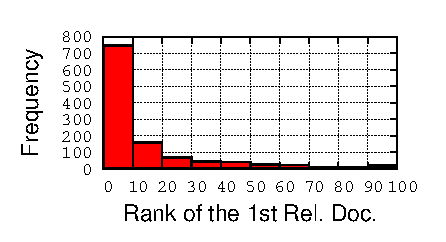
\includegraphics[width=5.5cm]{imgs/1stRank}
\par\end{centering}

\protect\caption{The distribution of the first relevant document rank over test queries.}
\label{fig:FirstTPRankHisto}
\end{figure}




\section{Related Work}
\label{Sec:RelatedWork}
% Reda: please have a look at this section and consider revising
%       as appropriate.  -Scott


Our work is different from pioneer studies on patent retrieval, as we
looked at the patent prior art problem from the term analysis perspective to figure out the main 
causes that generic IR methods do not work effectively in patent domain. 
%However, we cite here few works that focus mainly on query reformulation for patent search. 
In \cite{Itoh2003}, Itoh et al. proposed a new term selection method using different term
frequencies depending on the genre in the NTCIR-3 Patent Retrieval Task.
%Xue and Croft \cite{xue2009transforming} conducted a series of experiments in order to examine the effect of different patent fields, and concludes with the observation that the best MAP is achieved using the text from the description section. 
%Also, 
Fuji \cite{Fujii2007}
showed that retrieval effectiveness can be improved by combining IR
methods with the result of citation extraction.
Bashir et al. \cite{Bashir2010} proposed query expansion with pseudo-relevance
feedback that used machine learning for term selection.
%Terms are selected using a using a machine learning approach, by picking terms that may have a potential positive impact on the retrieval effectiveness. 
Verma and Varma
\cite{Verma2011} proposed a different approach, which instead of using
the patent text to query, use its IPC codes, which are expanded using the citation network.
% The formed query is used to perform an initial search. The results are then re-ranked using queries constructed from patent text.
%Magdy et al.~\cite{magdy2011study} studied works on query expansion 
%%in patent retrieval 
%and discussed that standard query expansion techniques are
%less effective, where the initial query is the full texts of query
%patents. 
Mahdabi et al.~\cite{Mahdabi2013} used term proximity
information to identify expansion terms. Ganguly et
al.~\cite{ganguly2011patent} adapted pseudo relevance feedback for
query reduction by decomposing a patent application into constituent
text segments and computing the Language Modelling (LM) similarities
of each segment from the top ranked documents. The least similar
segments to the pseudo-relevant documents removed from the query,
hypothesizing it can increase the precision of retrieval. Kim et
al.~\cite{kim2014diversifying} provided diverse query suggestion using
aspect identification from a patent query to increase the chance of
retrieving relevant documents. Magdy et al.~\cite{magdy2011study} studied 
%works on 
query expansion in patent retrieval 
and discussed that standard query expansion techniques are
less effective, where the initial query is the full texts of query
patents. 
%Mahdabi et al.~\cite{mahdabi2014patent}
%used linked-based structure of the citation graph together with IPC
%classification to improve the initial patent query. 
% Finally, other works investigated query suggestion for patent prior art search, which reflect real-life scenario of examiners, who form reproducible boolean queries \cite{Adams2011,Azzopardi2010,Kim2011}.












\begin{comment}
Our work is different from pioneer studies on patent retrieval, as we
closely looked into the problem rather than solutions to figure out
the causes that generic IR models which are based on term matching
process, do not work efficiently in patent domain. However, we cite here few works that focus mainly on query reformulation for patent search. 
In \cite{Itoh2003}, authors proposed a new term selection method using different term
frequencies depending on the genre in the NTCIR-3 Patent Retrieval Task.
Xue and Croft \cite{xue2009transforming} conducted a series of experiments
in order to examine the effect of different patent fields, and concludes
with the observation that the best MAP is
achieved using the text from the description section. Also, Fuji \cite{Fujii2007}
showed that retrieval effectiveness can be improved by combining IR
methods with the result of citation extraction.
Bashir et al. \cite{Bashir2010} propose query expansion with pseudo-relevance
feedback. Terms are selected using a using a machine
learning approach, by picking terms that may have a potential positive
impact on the retrieval effectiveness. Verma and Varma
\cite{Verma2011} propose a different approach, which instead of using
the patent text to query, use its IPC codes, which are expanded using the citation network. The formed
query is used to perform an initial search. The results are then re-ranked
using queries constructed from patent text.
Magdy et al.~\cite{magdy2011study} studied works on query expansion in patent
retrieval and discussed that standard query expansion techniques are
less effective, where the initial query is the full texts of query
patents. Mahdabi et al.~\cite{Mahdabi2013} used term proximity
information to identify expansion terms. Ganguly et
al.~\cite{ganguly2011patent} adapted pseudo relevance feedback for
query reduction by decomposing a patent application into constituent
text segments and computing the Language Modelling (LM) similarities
of each segment from the top ranked documents. The least similar
segments to the pseudo-relevant documents removed from the query,
hypothesizing it can increase the precision of retrieval. Kim et
al.~\cite{kim2014diversifying} provided diverse query suggestion using
aspect identification from a patent query to increase the chance of
retrieving relevant documents. Mahdabi et al.~\cite{mahdabi2014patent}
used linked-based structure of the citation graph together with IPC
classification to improve the initial patent query. 
Finally, other works investigated query suggestion for patent prior
art search, which reflect real-life scenario of examiners, who form
reproducible boolean queries \cite{Adams2011,Azzopardi2010,Kim2011}.
\end{comment}


% A ``Conclusion'' is not entirely necessary in a poster paper...
% include only if there is sufficient space.  -Scott%&\vfill\eject
\section{Conclusion}
\label{Sec:Conclusion}
\chapter{Conclusions}
\label{cha:conc}
%\textcolor{red}{Mona: I will compose this chapter after we confirmed about all chapters!}\\
%Summary your thesis and discuss what you are going to do in the future in Section~\ref{sec:future}.

%\section{Overview}
%\label{sec:overview}
%\section{Summary}
%\label{sec:summary}

In this thesis, we investigated the reasons that make patent prior art searches 
less effective than other web search applications.
% on CLEF-IP 2010 data collection. 
We started with recognising errors due to data curation and baseline settings that 
make only small portion of the whole errors. We hypothesized that the main portion of the errors is 
due to term matching process of retrieval ranking functions. 
Hence, we looked at the patent prior art search from
a term selection perspective. While previous studies proposed
different solutions to improve retrieval effectiveness, we 
focused on analysing terms in the patent query and top 100 retrieved patents. 
After defining an oracular query based on
relevance judgements, we established both the sufficiency
of the standard LM retrieval scoring models and query reduction 
methods to achieve state-of-the-art patent prior art
search performance. After finding that automated methods 
for query reduction approaches fail to offer significant
performance improvements, we showed that we can double
the MAP with minimum user interaction by approximating
the oracular query through a relevance feedback approach
with a single relevant document. Given that such simple 
interactive methods for query reduction with a standard LM
retrieval model outperform highly engineered patent-specific
search systems from CLEF-IP 2010, we concluded that interactive 
methods offer a promising avenue for simple but
highly effective term selection in patent prior art search.
 

\section{Contributions}
\label{sec:contributions}
We briefly summarise the major contributions of our work as follows:
\begin{enumerate}
\item \textbf{Development of an oracular term selection system: }We built an oracular term selection system from known relevance judgements to formulate an oracular query that far outperformed the baseline and the best-performed competitor on CLEF-IP 2010. 
Experiments related to the oracular system suggested the necessity of precise query
reduction and term selection techniques to improve the effectiveness of patent
prior art search.
\item \textbf{Analysis of automated query reduction techniques for patent prior art search: } We examined four simple query reduction methods to select the positive terms and to prune the negative terms out. We illustrated that these approaches were inefficient because they could not discriminate between useful terms and noisy terms. Since our system was over-sensitive to the existence of noisy terms, we could not achieve high performance via these simple methods. 
\item \textbf{Proposal of a semi-interactive method for query term selection: }We showed that a simple minimal interactive relevance feedback approach, where terms are selected by only the first retrieved relevant document performs as well as a highly engineered patent-specific system on CLEF-IP 2010. 
\end{enumerate}

\section{Future Work}
\label{sec:future}
In this research, we analysed the key reasons making generic IR methods ineffective for patent prior art through various experiments that may open further research on the topic of prior art search. We describe the limitations and discuss further improvements as follows: 
\subsection{Exploring Other Term Scoring Methods}
\label{subsec:ExploringTermScoringMethods}
Our term scoring method inspired by Rocchio optimal query~\citep{manning2008introduction}. We used this score to select query terms, which resulted in a remarkable improvement in the performance. However, exploring other existing term scoring techniques like Kullback-Leibler divergence~\citep{Baeza-Yates2011} may improve the results.
\subsection{Exploring More Sophisticated Query Reduction Methods}
\label{subsec:SophisticatedQueryReduction}
We demonstrated that useful terms in the patent query are sufficient for an effective retrieval.
We showed that a query, formulated by a precise selection of useful terms, considerably outperforms the baseline and PATARAS. We were unsuccessful in approximating the oracular query by automated techniques 
because the retrieval models are over-sensitive to noisy terms and our proposed reduction approaches were incapable of discriminating between useful terms and noisy terms. 
Hence, we need more sophisticated query term selection techniques, which differentiate useful terms from noisy terms. 
For example, query term selection technique, proposed by~\cite{maxwell2013compact} using affinity graph and random walk, can be applied for patent prior art search.     

\subsection{Considering Phrasal Concepts for Query Reformulation }
\label{subsec: PhraseAnalysis}
Our research was limited to only single terms in patent documents. 
However, one important characteristic of patents is that 
inventors use longer technical terms to describe their research ideas. 
Hence, phrasal concepts and terminology 
are frequently used as keywords in target patent documents.
Hence, an obvious extension of this work is extracting phrasal concepts while reformulating the query. 

\subsection{Patent Retrieval Using Meta-data Social Information}
\label{subsec: Meta-dataNetworkAnalysis}
A retrieval based on meta-data social information and social network analysis 
is a proper alternative to a traditional IR based on term matching process 
when the retrieval problem based on term matching is difficult.
Patents are rich in meta-data; for example 
the bibliographic meta-data in the patent XML file contains details about 
its inventor, organisation, and other information that can build a multidimensional graph.
Recent studies aim at improving the IR process with
information coming from social networks; this is commonly known as social IR. 
Regarding this social network structure of patents, we can  
find possible prior works in the social profile of other inventors with the same research interest.
Also competitive organisations may have developed the same or very close idea prior to the  
idea, which is claimed in the~patent~application.




%ACKNOWLEDGMENTS are optional
\section{Acknowledgments}
NICTA is funded by the Australian Government as represented by the Department of Broadband, Communications and the Digital Economy and the Australian Research Council through the ICT Centre of Excellence program.

% The following two commands are all you need in the
% initial runs of your .tex file to
% produce the bibliography for the citations in your paper.
\bibliographystyle{abbrv}
{\scriptsize
\bibliography{sigproc}
} % sigproc.bib is the name of the Bibliography in this case
% You must have a proper ".bib" file
%  and remember to run:
% latex bibtex latex latex
% to resolve all references
%
% ACM needs 'a single self-contained file'!
%
%APPENDICES are optional
%\balancecolumns
%\appendix
%%Appendix A
%\section{Headings in Appendices}
%The rules about hierarchical headings discussed above for
%the body of the article are different in the appendices.
%In the \textbf{appendix} environment, the command
%\textbf{section} is used to
%indicate the start of each Appendix, with alphabetic order
%designation (i.e. the first is A, the second B, etc.) and
%a title (if you include one).  So, if you need
%hierarchical structure
%\textit{within} an Appendix, start with \textbf{subsection} as the
%highest level. Here is an outline of the body of this
%document in Appendix-appropriate form:
%\subsection{Introduction}
%\subsection{The Body of the Paper}
%\subsubsection{Type Changes and  Special Characters}
%\subsubsection{Math Equations}
%\paragraph{Inline (In-text) Equations}
%\paragraph{Display Equations}
%\subsubsection{Citations}
%\subsubsection{Tables}
%\subsubsection{Figures}
%\subsubsection{Theorem-like Constructs}
%\subsubsection*{A Caveat for the \TeX\ Expert}
%\subsection{Conclusions}
%\subsection{Acknowledgments}
%\subsection{Additional Authors}
%This section is inserted by \LaTeX; you do not insert it.
%You just add the names and information in the
%\texttt{{\char'134}additionalauthors} command at the start
%of the document.
%\subsection{References}
%Generated by bibtex from your ~.bib file.  Run latex,
%then bibtex, then latex twice (to resolve references)
%to create the ~.bbl file.  Insert that ~.bbl file into
%the .tex source file and comment out
%the command \texttt{{\char'134}thebibliography}.
%% This next section command marks the start of
%% Appendix B, and does not continue the present hierarchy
%\section{More Help for the Hardy}
%The sig-alternate.cls file itself is chock-full of succinct
%and helpful comments.  If you consider yourself a moderately
%experienced to expert user of \LaTeX, you may find reading
%it useful but please remember not to change it.
%\balancecolumns % GM June 2007
% That's all folks!



\end{document}
